% ------------------------------------------------------------------------------
% OpenQuake Engine Book 
% 
% Authors: 
% 	H. Crowley 		- Executive Committee - GEM Foundation, Pavia, Italy
% 	D. Monelli 		- GEM Model Facility, ETH-SED, Zurich, Switzerland
% 	M. Pagani 		- Executive Committee - GEM Foundation, Pavia, Italy
% 	V. Silva 		- GEM Model Facility, Pavia, Italy
%	G. Weatherhill 	- GEM Model Facility, Pavia, Italy
% 
% Document distributed under the Common Creative License 
% © GEM Foundation, Pavia, February 2011
% ------------------------------------------------------------------------------
\documentclass[11pt,a4paper,headings=small,dvips]{scrbook}
% --------------------------------------------------------------------- Packages
\setcounter{secnumdepth}{3}
\setcounter{tocdepth}{3}
% This is used to create the cover and to plot trees
\usepackage{pst-tree}
\usepackage{pstricks,pstricks-add,multido}
%
\usepackage{geometry}
\usepackage{moresize}

\usepackage{chappg}

%
%\usepackage{algorithmic}
% 
\usepackage{fancyvrb}
\usepackage{listings}
\usepackage{alltt}
\usepackage{gensymb}
%
\usepackage[section]{placeins}
% 
\usepackage{pbox}
% http://en.wikibooks.org/wiki/LaTeX/Indexing
\usepackage{makeidx} 
\makeindex
%
%\usepackage{subfigure}
% Figure caption settings
\usepackage[textfont=it,margin=10pt,font=small,labelfont=bf,labelsep=endash]{caption}
\usepackage{subcaption}
%
\usepackage{bm}
% Landscape package
\usepackage{lscape}
%
\usepackage{hyperref} 
\hypersetup{colorlinks=true}
\hypersetup{breaklinks=true}
% package for multiline comments
\usepackage{verbatim}

\usepackage{xcolor}
\usepackage{framed}
\usepackage[utf8]{inputenc}

%
% Package to create a glossary - It must be uploaded after hyperref
% to produce the glossary: makeglossaries OQB
%\usepackage[toc,acronym,nonumberlist,style=altlist]{glossaries}
\usepackage[toc,nonumberlist,style=altlist]{glossaries}
\glstoctrue
\makeglossaries
%
% - - - - - - - - - - - - - - - - - - - - - - - - - - - - - - - - Setting Fonts
% \renewcommand{\encodingdefault}{OT1}
\renewcommand{\encodingdefault}{OT1}
\renewcommand{\familydefault}{ppl}
% \renewcommand{\familydefault}{cmss}
% \renewcommand{\seriesdefault}{m}
% \renewcommand{\shapedefault}{up}

% - - - - - - - - - - - - - - - - - - - - - - - - - - - - - - - - - - - - - - -
\usepackage{amsmath}
% - - - - - - - - - - - - - - - - - - - - - - - - - - - - - - - - - - - - - - -
\usepackage{titlesec}
\usepackage[dvips]{graphicx}
% - - - - - - - - - - - - - - - - - - - - - - - - - - - - - - - - - - - - - - -
\usepackage{type1cm,eso-pic,color}

%\makeatletter
%\AddToShipoutPicture{
%    \setlength{\@tempdimb}{.5\paperwidth}
%    \setlength{\@tempdimc}{.5\paperheight}
%    \setlength{\unitlength}{1pt}
%    \put(\strip@pt\@tempdimb,\strip@pt\@tempdimc){
%        \makebox(0,0){\rotatebox{55}{
%        	\textcolor[gray]{0.85}{
%        		\fontsize{5cm}{5cm}
%        		\selectfont{DRAFT}}
%        	}
%        }
%	}
%}
%\makeatother

%
% Solves problems with margin notes
\usepackage{mparhack} 
	\setlength{\marginparwidth}{1.1in}
	\let\oldmarginpar\marginpar
	\renewcommand\marginpar[1]{\-\oldmarginpar[\raggedright\color{red01}
	\footnotesize #1]%
	{\raggedright\footnotesize #1}}
% Define some colors
	\definecolor{azure}{RGB}{240,255,255}
	\definecolor{honeydew}{RGB}{240,255,240}
	\definecolor{blue01}{RGB}{4,64,116}
	\definecolor{blue02}{RGB}{0,62,113}
	\definecolor{gray01}{rgb}{0.1,0.1,0.1}
	\definecolor{gray02}{rgb}{0.8,0.8,0.8}
	\definecolor{red01}{rgb}{0.5,0.0,0.0}
	\definecolor{orange00}{rgb}{1.0,0.74,0.53}
	\definecolor{orange01}{rgb}{0.9137,0.5882,0.0980}
	\definecolor{orange02}{rgb}{0.7608,0.4157,0.1804}
	\definecolor{orange03}{rgb}{0.6941,0.1843,0.1333}
\usepackage[english]{babel}
% Bibliography settings
\usepackage[square,colon]{natbib} % Extend bibligraphy functions
% Page numbering by Chapter
%\usepackage[auto]{chappg} 
%\pagenumbering{bychapter}
% 
% Define page properties
\usepackage{scrpage2}
	\pagestyle{scrheadings}
	\lofoot[]{}
	\refoot[]{}
	%\lofoot[]{\includegraphics[width=1.0cm]{./figures/openquake_logo.eps}}
	%\refoot[]{\includegraphics[width=1.0cm]{./figures/openquake_logo.eps}}
	%\renewcommand{\partpagestyle}{empty}
% - - - - - - - - - - - - - - - - - - - - - - - - - -  Reformatting PART Titles
\titleformat{\part}[display]
{\filleft\normalfont\sffamily}
{\textcolor{blue01}{\bfseries\large PART}\hspace{4pt}
	\bfseries\Huge\textcolor{blue01}{\thepart}}
{1pc}
{\Huge\bfseries\textcolor{blue01}}
[]
% - - - - - - - - - - - - - - - - - - - - - - - - - Reformatting CHAPTER Titles
% Titles: CHAPTER
\titleformat{\chapter}
	[display] % shape
	{\filleft\normalfont\sffamily} % format
	{\textcolor{blue01}{\bfseries\MakeUppercase{\chaptertitlename}} % label
	\hspace{4pt}\huge\bfseries\textcolor{blue01}{\thechapter}} 
	{1pc} % sep
	{\huge\bfseries\textcolor{blue01}} % Before
	[]
% - - - - - - - - - - - - - - - - - - - - - - - - - Reformatting SECTION Titles
% Titles: SECTION
\titleformat{\section}
	[hang] % shape
	{\vspace{.8ex}\Large\bfseries\color{blue01}} % format 
	{\textcolor{blue01}{\thesection.}} % label
	{.5em} % sep
	{} % before
	[] % after
% - - - - - - - - - - - - - - - - - - - - - - -  Reformatting SUBSECTION Titles
% Title: SUBSECTION
\titleformat{\subsection}
	[hang] % shape
	{\vspace{.8ex}\large\bfseries\color{blue01}} % format 
	{\textcolor{blue01}{\thesubsection.}} % label
	{.5em} % sep
	{} % before
	[] % after
%  - - - - - - - - - - - - - - - - - - - - -  Reformatting SUBSUBSECTION Titles 
% Title: SUBSUBSECTION
\titleformat{\subsubsection}
	[hang] % shape
	{\vspace{.8ex}\normalfont\bfseries\color{blue01}} % format 
	{\textcolor{blue01}{\thesubsubsection.}} % label
	{.5em} % sep
	{} % before
	[] % after
% - - - - - - - - - - - - - - - - - - - - - - -  Reformatting PARAGRAPH Titles 
% Title: PARAGRAPH
\titleformat{\paragraph}
	[hang] % shape
	{\vspace{.2ex}\normalfont\color{blue01}} % format 
	{} % label
	{} % sep
	{} % before
	[] % after
%

%
% ------------------------------------------------------------------------------
\uppertitleback{
   \textbf{Authors:} \\
   Helen Crowley$^1$, Vitor Silva$^2$ \\ \hfill \\
   \small
   \begin{tabular}{p{4cm}p{4cm}p{4cm}}
   $^1$ GEM Foundation \hfill \newline
   via Ferrata, 1 \hfill \newline 
   20133 Pavia \hfill \newline
   Italy \hfill \newline
   & 
   $^2$ GEM Model Facility \hfill \newline 
   via Ferrata, 1 \hfill \newline 
   20133 Pavia \hfill \newline
   Italy \hfill \newline   
	\end{tabular} \hfill \newline
   %
	Email address (for all the authors):\hfill\\
   $<$name.surname$>$@globalquakemodel.org
   %
   \vspace{0.2cm} \hfill \\
   {\bf{Disclaimer}} \hfill \\
   The OpenQuake Engine Book is distributed in the hope that it will be useful, 
   but without any warranty: without even the implied warranty of 
   merchantability or fitness for a particular purpose. While every 
   precaution has been taken in the preparation of this document, in 
   no event shall the authors of the book and the GEM Foundation be 
   liable to any party for direct, indirect, special, incidental, or 
   consequential damages, including lost profits, arising out of the 
   use of information contained in this document or from the use of 
   programs and source code that may accompany it, even if the authors 
   and GEM Foundation have been advised of the possibility of such damage. 
   The Book provided hereunder is on as "as is" basis, and the authors 
   and GEM Foundation have no obligations to provide maintenance, support,
   updates, enhancements, or modifications. 
   \hfill \\
   The current version of the book has been revised only by members of 
   the GEM Model Facility and it must be considered a draft copy.
   %
   \vspace{0.2cm} \hfill \\
   {\bf{License}} \hfill \\
   This Book is distributed under the Creative Common License 
   Attribution 3.0 Unported (CC BY 3.0) 
   (see link below). You can download this Book and share it with others 
   as long as you provide proper 
   credit, but you cannot change it in any way.
   \hfill \\
   \href{http://creativecommons.org/licenses/by/3.0/}
   {http://creativecommons.org/licenses/by/3.0/}  
   
   \hfill \\
   {\bf{Credit}} \hfill \\
   Crowley, H., V. Silva (2013). OpenQuake Engine Book: Risk v1.0.0. GEM Foundation, Pavia, Italy.   
   \normalsize
}  
%
% =============================================================== BEGIN DOCUMENT
% -------------------------------------------------- Title and table of contents
\begin{document}
% - - - - - - - - - - - - - - - - - - - - - - - - - - - - - - - - - - - -  Cover
\newgeometry{hmargin={-0.4cm,0cm},height=29.7cm}
\thispagestyle{empty}
\psset{unit=1cm}
\begin{pspicture}(0,0)(21cm,29.7cm)
	\psframe[fillstyle=solid,linecolor=white,fillcolor=white]
		(0.0cm,15.0cm)(21cm,29.7cm)	
	\rput[l](0cm,14.85cm){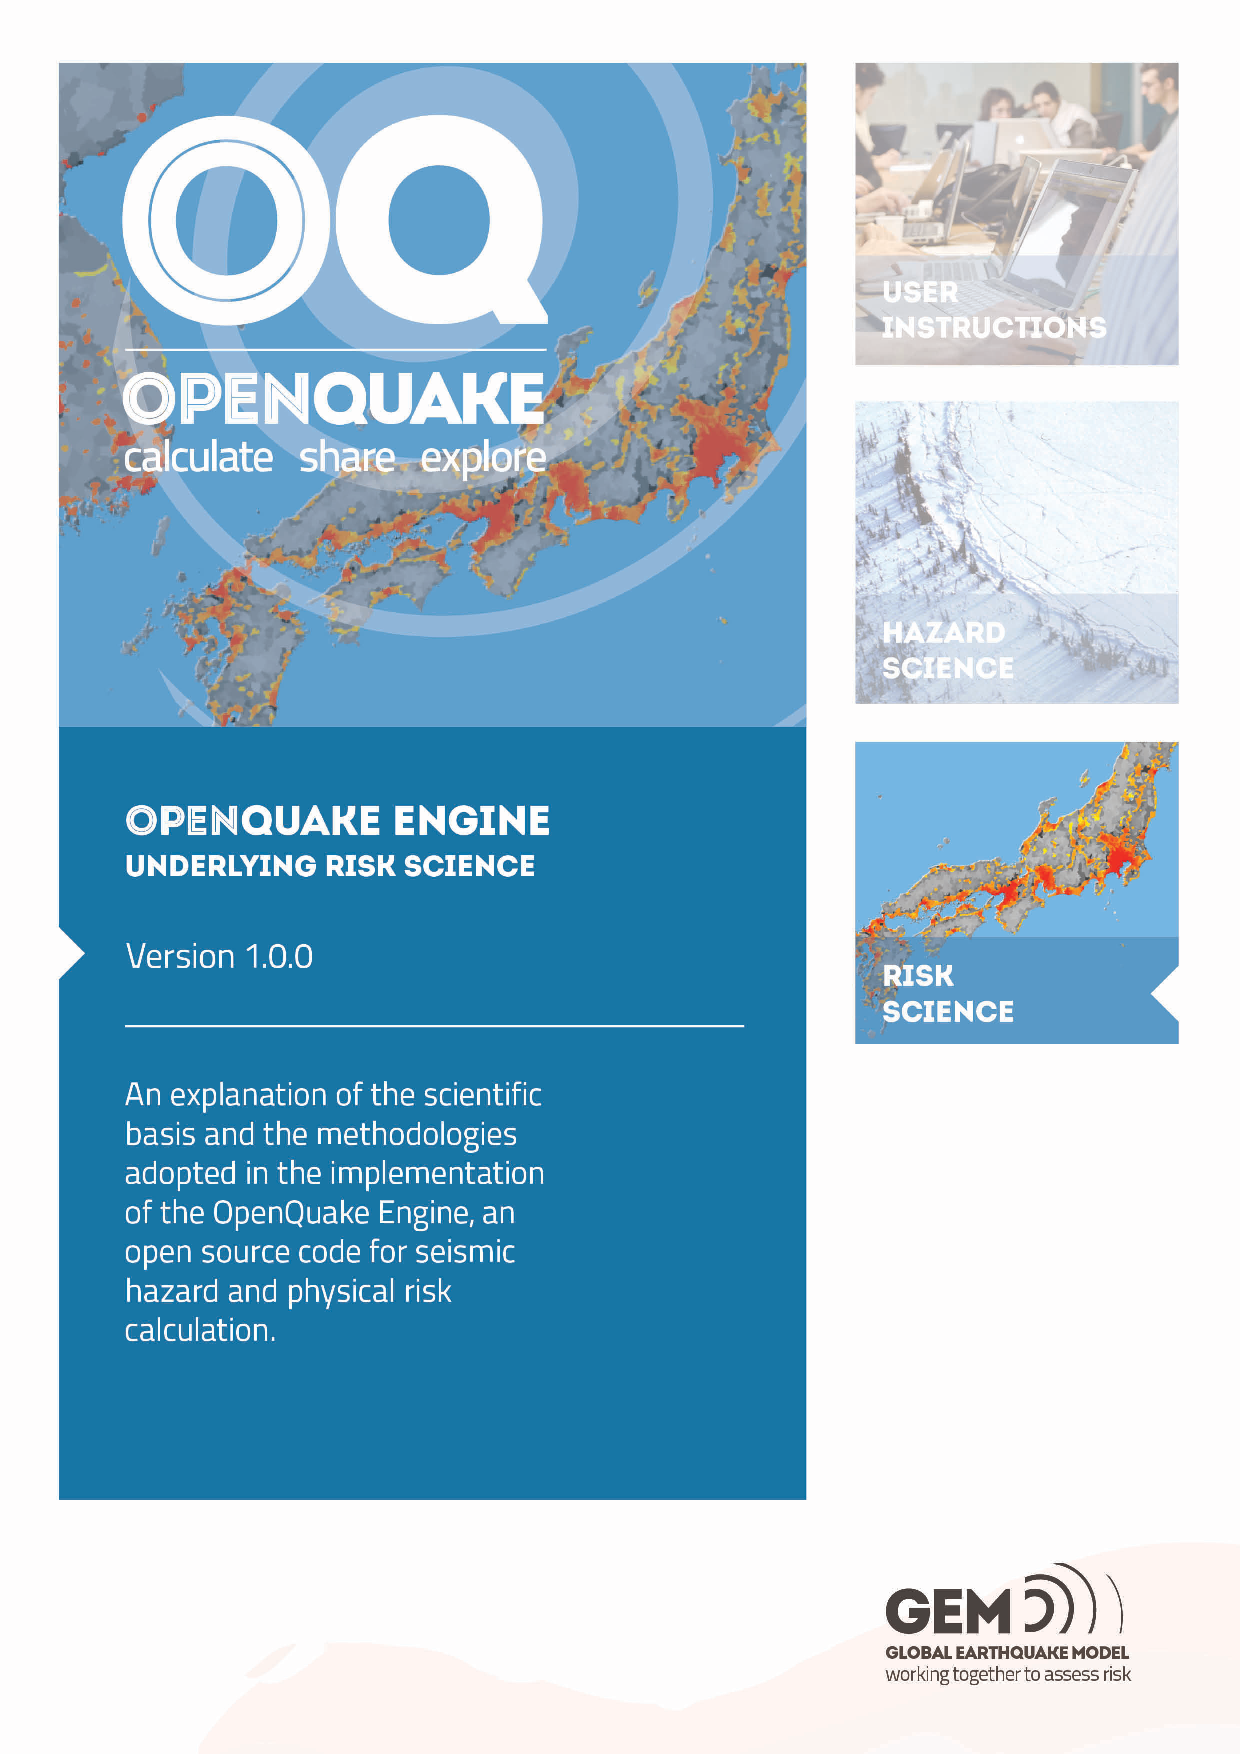
\includegraphics[width=21cm,height=29.7cm]{./figures/risk_cover.eps}}
	% Title
		% Logos
	
%	\rput(4cm,27.5cm){\includegraphics[height=2.0cm]
%		{./Figures/openquake_logo1.eps}}
	%
%	\rput[r](19.5cm,2cm){\sffamily\large\color{cyan}{Version 0.9}}
\end{pspicture}
%  - - - - - - - - - - - - - - - - - - - - - - - - - - - - - - - - - Second page
\restoregeometry
\thispagestyle{empty}
\cleardoublepage
% - - - - - - - - - - - - - - - - - - - - - - - - - - - - - -  Load the glossary
% OpenQuake Book Glossary 
% To cite a glossary element in a document:
%	\gls{seismicsourcedata}
%	\Gls{seismicsourcedata} - First initial is uppercase
%	\GLS{seismicsourcedata} - All initials are uppercase
%	\glspl{seismicsourcedata} - Plural
% To process the glossary:
% 	makeglossaries oqb

%
% ------- A
\newglossaryentry{areasource}{
	name = area source,
	description={A source type usually adopted to model distributed 
	seismicity. In an area source the seismicity occurrence rate 
    is assumed uniform over the source area; this produces an hazard 
    pattern with a plateau of constant hazard inside the polygon 
    delimiting the area source and values of hazard that tend to 
    decrease as we move away from the border of the source}
}
\newglossaryentry{asset}{
    name = asset,
    description={An asset is something of value, which can include 
    buildings and population. For example, an asset can include an 
    individual building at a given location, or a number of buildings 
    that are grouped and co-located at a single location 
    and are classified with the same \gls{taxonomy}} 
}
%
% ------- B
\newglossaryentry{branch}{
	name = branch,
	plural= branches,
	description={
	The simplest element in a logic tree; it belongs to a 
	\gls{branchset} where it represents one possible option among a finite 
	number of alternatives. A branch is associated with a weight 
	value \citep{scherbaum2011} if the \gls{branchset} represents the 
	epistemic uncertainty on a parameter or a model when the \gls{branchset} 
	is used to specify alternative models (e.g. district \glspl{acr:fmd})}
}
\newglossaryentry{branchinglevel}{
	name = branching level,
	description={It indicates the position where a \gls{branchset} or a 
	\gls{branch} is located in a logic tree structure. For example, 
	in \gls{acr:oq} the first branching level of the 
	\gls{seismicsourcelogictree} always contains one or several 
	\glspl{initialseismicsourcemodel}
	}
}
\newglossaryentry{branchset}{
	name = branch set,
	description={The structure describing the epistemic uncertainty on 
	a specific parameter or model included in a logic tree structure. 
	It ensembles a number of \glspl{branch}, each one representing a 
	discrete alternative}
}
%
% ------- C
\newacronym{cpsha}{cPSHA}{Classical PSHA}
\newglossaryentry{configurationfile}{
	name =  configuration file,
	description = {
	Usually the file containing the information necessary to run a calculation
	in OpenQuake}
}
\newglossaryentry{charfaultsource}{
	name = characteristic fault source,
	description={
	A fault source typology where ruptures always cover the entire fault surface
	}
}
\newglossaryentry{complexfaultsource}{
	name = complex fault source,
	description={
	A source typology usually adopted to model subduction interface faults, 
    where ruptures can be floated over the fault surface}
}
\newglossaryentry{consequence function}{
	name = consequence function,
	description={
	Consequence functions describe the probability distribution of loss, given a performance level and are generally derived empirically}
} 
%
% ------- D
\newglossaryentry{seismichazarddisaggregation}{
	name =  seismic hazard disaggregation,
	description = {
	A methodology to investigate the contributions to a specific
	level of hazard in terms of fundamental variables commonly used
	to characterize seismic sources and ground motion models (e.g. 
	magnitude, source-site distance, \gls{epsilon}}
}
\newglossaryentry{dip}{
	name = dip,
	description={
    The dip is the steepest angle of descent of the fault plane
    relative to a horizontal plane; it is measured in degrees [0,90] 
	}
}
\newglossaryentry{disaggregationmatrix}{
	name =  disaggregation matrix,
	description = {
	A multi-dimensional matrix used to systematically store the contributions
	to a level of hazard to be disaggregated and that is specified by the 
	user.
	See also \gls{seismichazarddisaggregation}}
}
%
% ------- E
\newacronym{acr:erf}{ERF}{Earthquake\- Rup\-ture\- Forecast}
\newacronym{acr:epsha}{ePSHA}{Event-based PSHA}
%
\newglossaryentry{earthquakeruptureforecast}{
	name = earthquake rupture forecast,
	description={
	A list of all possible ruptures generated by all the sources included 
	in a seismic source model. Each element in the list contains: the rupture 
	geometry and the rupture probability of occurrence in a given time span. 
	%
	See also the definition available on the 
	\href{http://www.opensha.org/glossary-earthquakeRuptureForecast}
	{OpenSHA website}}
}
\newglossaryentry{earthquakeruptureforecastcalculator}{
	name = earthquake rupture forecast calculator,
	description={
	Calculator producing a \gls{seismicsourcemodel} from a 
	\gls{seismicsourcelogictree} 
	}
}
%
\newglossaryentry{epsilon}{
	name = epsilon,
	description={
	normalized residual of the ground motion}
}
\newglossaryentry{exposure model}{
	name = exposure model,
	description={
	A set of \glspl{asset} grouped according to their geographical location, 
	\gls{taxonomy} and value}
}	
%
% ------- F
\newglossaryentry{faulttrace}{
	name = fault trace,
	description={A curve representing the intersection between the surface 
    representing the fault and the topographic surface
    \begin{figure}[!h]
    \centering
    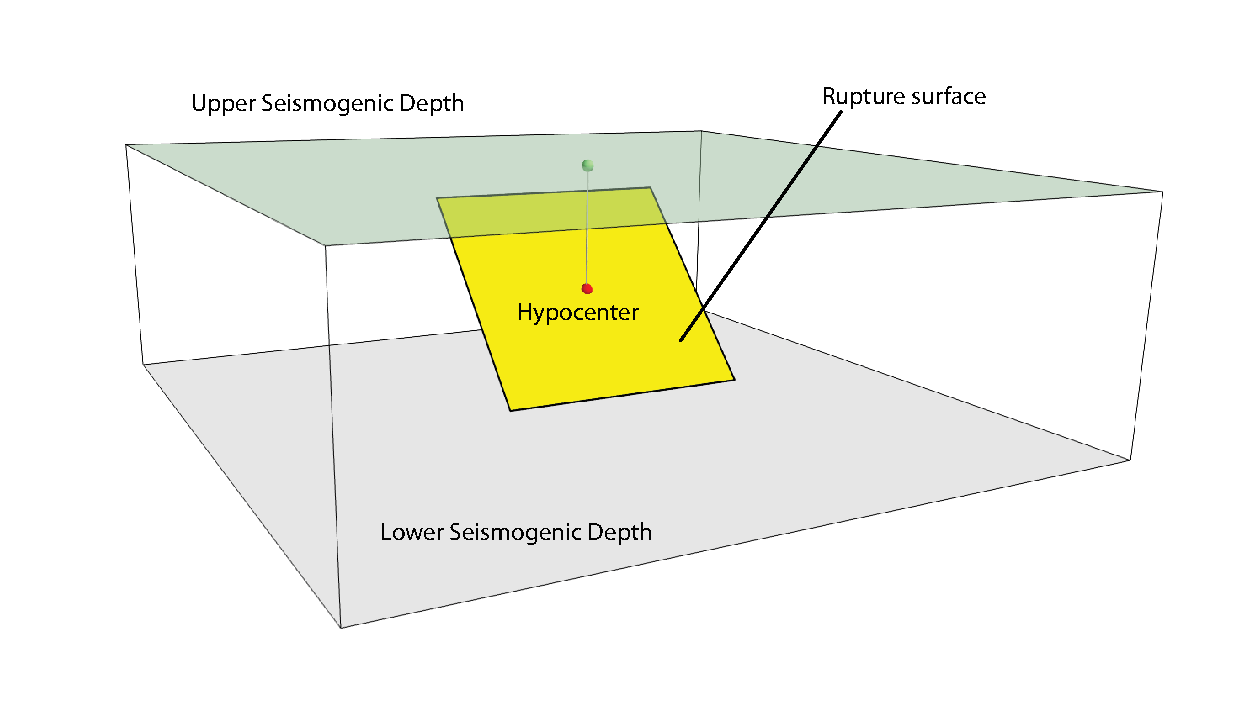
\includegraphics[width=10cm]{./figures/hazard/single_rupture.eps}
    \caption{Trace example}
    \label{fig:trace}
    \end{figure}
    }
}
\newglossaryentry{fragility function}{
	name = fragility function,
	description = {the probability of exceeding a set of limit states, 
	given an intensity measure level. These functions can be discrete or
	continuous}
}
\newglossaryentry{fragility model}{
	name = fragility model,
	description = {A set of \glspl{fragility function} used to model the 
	fragility of all the \glspl{asset} in the \gls{exposure model}.}
}
\newglossaryentry{frequencymagnitudedistribution}{
	name = magnitude-frequency distribution,
	description = {See \gls{mfd}
	}
}
%
% ------- G
\newacronym{acr:gem}{GEM}{Global Earthquake Model}
\newacronym{acr:gmpe}{GMPE}{Ground Motion Prediction Equation}
\newacronym{acr:gmlt}{GMLT}{Ground Motion Logic Tree (see 
    \gls{groundmotionlogictree}} 
\newglossaryentry{gridsource}{
	name = grid source,
	description={
	It's a source typology usually adopted to model distributed 
	seismicity. It's usually produced by a seismicity smoothing algorithm 
	(one of the most famous algorithm is the one proposed by 
	\citet{frankel1995})}
}
\newglossaryentry{groundmotionfield}{
	name = ground-motion field,
	description={An object describing the geographic distribution around 
	a rupture of a ground motion intensity measure}
}
\newglossaryentry{groundmotionfieldcalc}{
	name = ground-motion field calculator,
	description={An \gls{acr:oq} calculator that given a rupture computes the 
	geographic distribution of a ground motion intensity parameter. Currently
	OQ can generate ground motion fields using a \gls{acr:gmpe}}
}
\newglossaryentry{groundmotionlogictree}{
	name = ground-motion logic tree,
	description={A method used to systematically describe the epistemic 
	uncertainties related to the ground motion models used in the 
	computation of hazard using a specific \gls{pshainputmodel}}
}
\newglossaryentry{groundmotionmodel}{
	name = ground-motion model,
	description={An object that given a rupture with specific properties
	computes the expected ground motion at the given site. In simplest case 
	a ground motion model corresponds to a \gls{groundmotionpredictioneq}. 
	In case of complex PSHA input models, the produced ground motion models 
	contains a set of \glspl{acr:gmpe}, one for each tectonic region considered.
	}
}
\newglossaryentry{groundmotionparameter}{
	name = ground-motion parameter,
	description={A scalar or vector quantity describing a relevant property
	of the shaking such as intensity (e.g. PGA or Spectral Acceleration) 
	or duration, equivalent number of cycles 
	\citep[see for example][]{hancock2005})
	}
}
\newglossaryentry{groundmotionpredictioneq}{
	name = ground-motion prediction equation,
	description={
		An equation that - given some fundamental parameters characterizing 
		the source, the propagation path and the site (in the simplest 
		case magnitude, distance and V$_\text{S,30}$) - computes the 
		value $GM$ of a (scalar) ground motion intensity parameter.
	}
}
\newglossaryentry{groundmotionsystem}{
	name = ground-motion system,
	description={An object containing a list of \gls{groundmotionlogictree}}
}
%
% ------- I 
\newglossaryentry{initialseismicsourceinputmodel}{
	name = initial seismic source input model,
	description={An initial seismic source input model is a 
    \gls{seismicsourceinputmodel} included in the first 
	branching level of a seismic source logic tree}
}
\newglossaryentry{investigationtime}{
	name = investigation time,
	description={The time interval considered to calculate hazard; usually 
	it corresponds to 50 years}
}
%
% ------- L
\newglossaryentry{logictree}{
	name = logic tree,
	description={Data structure used to systematically describe uncertainties
	on parameters and models used in a PSHA study}
}
\newglossaryentry{logictreeprocessor}{
	name = logic tree processor,
	description={An OQ calculator that takes the PSHA Input Model and creates 
	many realisations of a \gls{seismicsourcemodel} and of a 
	\gls{groundmotionmodel}}
} 
\newacronym{acr:ltmcs}{LTMCS}{Logic Tree Monte Carlo Sampler}
%
%
\newglossaryentry{msr}{
    name = magnitude-scaling relationship,
    description={
        An empirical relationship linking the magnitude with a parameter
        describing the size of the corresponding rupture (e.g. the area 
        of the rupture or the rupture length)
    }
}
\newacronym{acr:mfd}{MFD}{Magnitude-Frequency Distribution}
\newglossaryentry{mfd}{
    name = magnitude-frequency distribution,
    description={
   	    A distribution describing the frequency of earthquakes with 
        a specific magnitude. It can be continuous or discrete. 
        One frequency-magnitude distribution frequently adopted in 
        \gls{acr:psha} is the double truncated Gutenberg-Richter 
        distribution
    }
}
%
% ------- O
\newacronym{acr:hazlib}{oq-hazardlib}{OpenQuake hazard library}
\newglossaryentry{opensha}{
	name = OpenSHA,
	description = {OpenSHA is an open-source, advanced Java-based 
	platform for conducting Seismic Hazard Analysis - 
	(see \href{http://opensha.org}{OpenSHA website}). \gls{acr:oq}-hazard 
	relies on a distilled version of OpenSHA}
}
\newacronym{acr:oq}{OQ}{OpenQuake}
\newacronym{acr:oqe}{OQe}{OpenQuake-engine}
%
% ------- P
\newacronym{acr:pga}{PGA}{Peak Ground Acceleration}
\newacronym{acr:pgv}{PGV}{Peak Ground Velocity}
\newacronym[description={\glslink{psha}{Probabilistic 
    Seismic Hazard Analysis}}]{acr:psha}{PSHA}{Probabilistic Seismic 
    Hazard Analysis}
\newglossaryentry{pointsource}{
	name=point source, 
	description={The elemental source typology used in OpenQuake-engine to 
	model distributed seismicity}	
}
\newglossaryentry{pshainputmodel}{
	name=PSHA input model, 
	description={An object containing the information necessary to describe 
	the seismic source and the ground motion models - plus the related 
	epistemic uncertainties}	
}
\newglossaryentry{psha}{
	name = probabilistic seismic hazard analysis, 
	description={A methodology to compute seismic hazard by taking into 
	account the potential contributions coming from all the sources 
	of engineering importance for a specified site}	
}
%
% ------- R
\newacronym{acr:rjb}{r$_{\text{jb}}$}{Joyner and Boore distance}
\newglossaryentry{rupture}{
	name=earthquake rupture, 
	description={A 3D surface - representing a portion or the entire 
    fault surface - over which a slip event (i.e. an earthquake) 
    occurs.
	}	
}
\newglossaryentry{rake}{
	name=rake, 
	description={The rake is the angle 
	}	
}
%
% ------- S
\newacronym{acr:ssha}{SSHA}{Scenario Based Seismic Hazard Analysis}
\newglossaryentry{scenariohazard}{
	name = scenario based seismic hazard analysis,
	plural= scenario based seismic hazard analyses,
	description = {An analyis of seismic hazard based on the selection of
        one or a few ruptures and the computation of the expected ground 
        motion at a set of sites using a \gls{gmpe} accounting ground motion
        variability.
	}
}
\newglossaryentry{seismicityhistory}{
	name = seismicity history,
	plural= seismicity histories,
	description = {An object containing a set ruptures  
	representative of the possible seismicity generated by the 
	sources in a \gls{seismicsourcemodel} during the investigation 
	time $t$
	}
}
\newglossaryentry{seismicityrate}{
	name = seismicity rate,
	description = {Number of events per unit of time (if not better 
	specified, the definition of a seismicity rate generally presumes 
	a time independent 
	}
}
\newglossaryentry{seismicsourcedata}{
	name = seismic source data,
	description={An object containing the information necessary 
	to completely describe a \gls{acr:psha} seismic source i.e. seismic 
	source type, position, geometry and seismicity occurrence 
	model}
}
\newglossaryentry{seismicsourcelogictree}{
	name = seismic source logic tree,
	description={Logic tree structure defined to describe in 
	structured and systematic way the epistemic uncertainties 
	characterizing the seismic source model. The first 
	branching level in the logic tree by definition contains one or
	several alternative \gls{initialseismicsourcemodel}}
}
\newacronym[description={\glslink{seismicsourceinputmodel}{Seismic 
    Source Input Model}}]{acr:ssim}{SSIM}{Seismic Source Input Model}
\newglossaryentry{seismicsourceinputmodel}{
	name = seismic source input model,
	description={A collection of seismic source input. 
    In the OpenQuake-engine a seismic source model doesncontain 
    epistemic uncertainty}
}
\newacronym{acr:ssm}{SSM}{Seismic Source Model}
\newglossaryentry{seismicsourcemodel}{
	name = seismic source model,
	description={Technically a collection of SeismicSource objects
        (see \href{SeismicSource} 
        {https://github.com/gem/oq-hazardlib/blob/master/openquake/hazardlib/source/base.py})
    }
}
\newacronym{acr:scec}{SCEC}{Southern California Earthquake Center}
\newglossaryentry{seismicsourcesystem}{
	name = seismic source system,
	description={An object containing a list of \glspl{initialseismicsourcemodel}
	and the \gls{seismicsourcelogictree}}
}
\newglossaryentry{simplefaultsource}{
	name = simple fault source,
	description={
	A source typology usually adopted to model shallow structures with an
	uncomplicated geometry
	}
}
\newacronym{acr:ses}{SES}{Stochastic Event Set}
\newglossaryentry{stochasticeventset}{
	name = stochastic event set,
	description={An object containing one or many \glspl{seismicityhistory} 
	}
}
\newglossaryentry{strike}{
	name = strike,
	description={The strike
	}
}
\newacronym{acr:sa}{S$_a$}{Spectral Acceleration}
%
% ------- T
\newglossaryentry{taxonomy}{
	name = taxonomy,
	description = {Scheme used to classify the \glspl{asset}. For buildings,
	a classification scheme has been proposed by \gls{acr:gem} which considers
	a number of attributes including lateral load resisting system and its 
	material, height, year of construction. The taxonomy is currently used to 
	link the \glspl{asset} in the \gls{exposure model} to the relevant 
	\gls{vulnerability function} or \gls{fragility function}}
}
\newglossaryentry{tectonicregion}{
	name = tectonic region,
	description = {A area on the topographic surface that can be considered 
	homogeneous in terms of tectonic properties such as the prevalent 
	seismogenic properties and/or the seismic wave propagation properties
	}
}
\newglossaryentry{temporaloccurrencemodel}{
	name = temporal occurrence model,
	description = {Usually a probabilistic model giving the probability of
	occurrence of an event in a specified \gls{investigationtime}
	}
}
%
% ------- U
\newacronym{acr:usgs}{USGS}{United States Geological Survey}
%
% ------- V 
\newglossaryentry{acr:vs30}{
	name = V$_{S,30}$,
	description = {Average shear wave velocity of the 
	materials in the uppermost 30m of the soil column}
}
\newglossaryentry{vulnerability function}{
	name = vulnerability function,
	description = {A function that describes the probability distribution
	of loss ratio, conditioned on an intensity measure level. Currently only 
	discrete vulnerability functions are supported}
}
\newglossaryentry{vulnerability model}{
	name = vulnerability model,
	description = {A set of \glspl{vulnerability function} used to model the 
	physical vulnerability of all the \glspl{asset} in the \gls{exposure model}.}
}

%
% - - - - - - - - - - - - - - - - - - - - - - -  This is the internal title page
\setcounter{page}{1}
\begin{titlepage}
	\titlehead{\emph{``OpenQuake: Shaken not stirred''}}
	\title{ \textcolor{blue01}{\textsf{\bfseries\Huge OpenQuake Engine Book: Risk}}  }
	\date{July 2013}
	\publishers{GEM Foundation, Pavia}
\end{titlepage}
\pagestyle{scrheadings}
\maketitle
%
\chapter*{Acknowledgements}
A number of internal and external collaborators contributed to 
the development of the OpenQuake engine and their input is herewith acknowledged. 
As of version 1.0 (25th June 2013), these were the current and former GEM Model Facility Team members (Zurich, Switzerland,
and Pavia, Italy): \hfill \\
\hfill \\
\hfill \\
\begin{tabular}{l}
Lars Butler \\
Andrea Cerisara \\
Fabian Euchner \\
Anton Gritsay \\
Paul Henshaw \\
Muharem Hrnjadovic \\
Christopher MacGown \\
Joshua McKenty \\
Marco Milanesi \\
Matteo Nastasi \\
Luigi Panzeri \\
Michele Simionato \\
John Tarter \\
Giuseppe Vallarelli \\
Ben Wyss \\
\end{tabular} \hfill \\
%
%\hfill \\
%\hfill \\
%USGS OpenSHA Team (Denver, Colorado) \hfill \\
%\hfill \\
%\begin{tabular}{l}
%Ned Field \\
%Kevin Milner \\
%Peter Powers \\
%\end{tabular}


\cleardoublepage
%  
\tableofcontents
%
% --------------------------------------------------------- Symbols and acronyms
% \chapter*{Symbols and Acronyms}
%	\begin{tabular}{p{9.5cm}ll}
\bf{Quantity or Description} & \bf{Symbol or} & \bf{Unit of} \\ 
              & \bf{acronym}   & \bf{measure}  \\
Classical Probabilistic Seismic Hazard Analysis \dotfill & cPSHA & \\
Distance \dotfill & $R$ or $r$ & \text{km} \\ 
Event-based Probabilistic Seismic Hazard Analysis \dotfill & ePSHA & \\
Frequency-Magnitude Distribution \dotfill & FMD & \\
Gutenberg-Richter (frequency-magnitude distribution) \dotfill & G-R &  \\
Ground Motion (GM) or Intensity Measure Type (IMT) \dotfill & $U$ or $u$ & g \\
Ground Motion Field \dotfill & GMF & \\
Ground Motion Prediction Equation \dotfill & GMPE &  \\
Ground Motion Prediction Equation System \dotfill & GMPEsy &  \\
Magnitude \dotfill & $M$ or $m$ & \\
Natural hazards Risk Markup Language \dotfill & NRML & \\
Occurrence Rate \dotfill & $\lambda$ & events/yr \\
OpenQuake \dotfill & OQ & \\
Probabilistic Seismic Hazard Analysis \dotfill & PSHA & \\
PSHA Input Model \dotfill & PSHAim & \\
Rupture \dotfill & $rup$ & \\
Seismic Sources System \dotfill & SSsy \\
Stochastic Event Set \dotfill & SES & \\
\end{tabular}

% ==============================================================================
% ------------------------------------------------------------------------- Part
%\thispagestyle{empty}
%\part{Introduction}
% ------------------------------------------------------------------------------
\chapter{Motivation and Basics of the OpenQuake Engine}
	This book aims to provide an explanation of the scientific basis 
and the methodologies adopted in the implementation of the OpenQuake engine, an open source code for seismic hazard and physical risk calculation. 
%
The book follows the traditional openness and transparency features of the 
\gls{acr:gem} as clearly indicated in the development principles of 
the OpenQuake engine. 

%
The \gls{acr:gem} initiative is a global collaborative effort with the aim to provide organisations and people with tools and resources for transparent assessment of earthquake risk anywhere in the world.
%
The OpenQuake engine is a fully integrated, flexible and scalable hazard and physical risk 
calculation engine whose development is at the core of \gls{acr:gem}'s
overall objectives.
% ------------------------------------------------------------------------------
\section{Basics of the Engine}
The implementation of the OpenQuake software officially started in Summer 2010 
following the experience gained in \gls{acr:gem}'s kick-off project GEM1 
\citep{gemfoundation2010}, during which an extensive appraisal of existing hazard 
and physical risk codes was performed \citep{danciu2010,crowley2010}
and prototype hazard and risk software were selected, designed and
implemented \citep{pagani2010,crowley2010a}.

The current version of the OpenQuake engine is Python code developed 
following the most common requirements of Open Source 
software development, such as a public repository, IRC channel and open mailing lists. 
The source code, released under an open source software license,
is freely and openly accessible on a web based repository 
(see \href{http://github.com/gem}{github.com/gem}) while the 
development process is managed so that the community can participate 
to the day by day development as well as in the mid- and long-term 
design process. 
%
The software development also leverages on a number of open source projects 
such as \href {http://celeryproject.org}{Celeryd} and \href{http://www.rabbitmq.com}{RabbitMQ}, just to mention a few.

The hazard component of the engine largely relies on classes belonging to the OpenQuake Hazard library (see \href{https://github.com/gem/oq-hazardlib}{oq-hazardlib}) a comprehensive library for performing state-or-the-art PSHA. This library has been designed and implemented following the successful collaboration and important lessons learnt working with the \href{http://www.opensha.org}{OpenSHA} software and the developing teams at \gls{acr:usgs} and 
\gls{acr:scec} in GEM1. 
%
The risk component of the engine was designed in GEM1, prototyped in Java and eventually
coded in Python by the team operating at the \gls{acr:gem} 
Model Facility. This scientific code was originally integrated with the engine, but in late 2012 it was extracted to form the OpenQuake Risk Library (see \href{https://github.com/gem/oq-risklib}{oq-risklib}).

%A schema that illustrates the structure of the engine is 
%represented in Figure \ref{fig:openquake_schema}; the schema contains:
%purple boxes representing the main modules of the hazard component, 
%green boxes showing the modules of the risk component, white boxes
%with main outputs computed by the distinct modules and orange rectangles
%displaying the main input information that should be entered into the calculation engine. 
%
% ------------------------------------------------------------------------------
%\subsection{Brief description of the OpenQuake IT architecture}
%% ------------------------------------------------------------------------------
Openquake is the core of the OpenGEM system. 
%
As it appears in Figure \ref{fig:oq_it}, OpenQuake is powered by a 
number of open source software projects, of which OpenSHA-lite and 
RiskLib are currently the most essential ones. 
OpenSHA-lite is a ‘light’ version of the comprehensive software for 
probabilistic seismic hazard assessment OpenSHA and whose code serves
as a basis for the hazard component of the OpenQuake engine. RiskLib 
is a global collaboration project that is aimed at common development 
of a code ‘library’ for the risk all types of natural hazards, including
an API, on wh ich ‘apps’ can be built, such as tools that support risk
mitigation/reduction. The World Bank’s GFDRR, OpenGeo, AIFDR and GEM 
jointly work on RiskLib and its code repository, currently part of 
the OpenQuake project, will be broken out soon.
%
% . . . . . . . . . . . . . . . . . . . . . . . . . . . . . . . . . . . > Figure
\begin{figure}
\includegraphics[width=\textwidth,angle=0]{./Figures/Part_Introduction/oq_system_architecture.eps}
\caption{Openquake system architecture.}
\label{fig:oq_it}
\end{figure}
% . . . . . . . . . . . . . . . . . . . . . . . . . . . . . . . . . . . < Figure
%
Implementation of a standard format for data exchange for natural hazard
and risk,  is closely related to what is described above. The NRML 
(Natural hazards’ Risk Markup Language) format has been developed, which
is capable of encompassing a wide variety of risk and hazard data formats.
More information can be found in the detailed background documentation 
for OpenQuake.

The data services that are mentioned above are globally accessible 
read/write collaborations of core data sets that are exposed with a 
REST API. Some of the core modules of GEM will be available through 
the services and are currently being developed by GEM’s Model Facility 
development team, in collaboration with a number of IT partners and the 
scientists coordinating the modules. Examples are the development of a 
global exposure database, development of a global portal for active 
faults, global vulnerability functions and an earthquake consequences
database.






%
% ------------------------------------------------------------------------------
\section{Structure of the Book}
The OpenQuake Engine Book is organized into two volumes, one which describes the science behind the hazard component of the engine
and another which illustrates the theory of the physical risk calculators incorporated into the software. Readers that are interested in learning how to run calculations using the OpenQuake engine are referred to the OpenQuake Engine User Manual.

\hfill \\
%\emph{Part II: Hazard}
The GEM Hazard Team is currently updating the volume on hazard. In the meantime, interested readers are referred to the OpenQuake Engine User Manual, or they can contact the coordinator, Dr Marco Pagani, for further information. 
%\begin{itemize}
%\item Chapter \ref{chap:inthaz} offers an introduction to the hazard 
%topics discussed in the following chapters. In particular, in this 
%Chapter we discuss the main OpenQuake concepts and we illustrate the 
%calculation workflows currently available in the hazard component of 
%OpenQuake.
%\item Chapter \ref{chap:hazinp} focuses on the structure and the 
%characteristics of the information necessary to define a 
%comprehensive PSHA input model. This Chapter also includes
%descriptions of the main seismic source typologies and of the logic 
%tree structure.
%\item We dedicate Chapter \ref{chap:erf} to the explanation of the
%methodology adopted for the processing of the logic tree structures
%supported by OpenQuake and for the creation of the 
%\gls{earthquakeruptureforecast}
%\item The last Chapter of the hazard part (chapter \ref{chap:hazcalc}) 
%illustrates the main calculators available: the classical-PSHA calculator,
%the event-based calculator and the disaggregation calculator. 
%\end{itemize}
\hfill \\
\hfill \\
%\emph{Part III: Risk}
This volume on risk is organised as follows:
\begin{itemize}
\item Chapter \ref{chap:intrisk} introduces the main physical risk concepts and workflows. 
\item Chapter \ref{chap:riskinput} contains an explanation of the exposure, physical vulnerability and fragility concepts, which are input to the calculations.
\item Chapter \ref{chap:scenario_risk} describes the scenario risk 
methodology, for estimating loss distributions for single events.
\item Chapter \ref{chap:scenario_damage} describes the scenario damage 
methodology, for estimating damage ditributions for single events.
\item Chapter \ref{chap:risk_prob_event_based} provides an overview of the probabilistic event-based risk calculation methodology, which produces loss exceedance curves for portfolios of buildings.
\item Chapter \ref{chap:risk_psha_based} illustrates single-site risk calculations based on the hazard curves from classical PSHA.
\item Chapter \ref{chap:bcr} outlines the benefit/cost ratio calculations based on loss curves for structures with and without retrofitting.
\end{itemize}
%
%In the closing part, the Book contains a glossary that aims to define a 
%clear and unique terminology.
%
% . . . . . . . . . . . . . . . . . . . . . . . . . . . . . . . . . . . > Figure
%\begin{landscape}
%\begin{figure}
%\includegraphics[width=20cm,angle=0]{./Figures/Part_Introduction/engine9_20110130.eps}
%\caption{OpenQuake Engine schema. Purple boxes are the calculators included in the  
%the hazard part of OQ; green boxes are the physical risk calculators.}
%\label{fig:openquake_schema}
%\end{figure}
%\end{landscape}
% . . . . . . . . . . . . . . . . . . . . . . . . . . . . . . . . . . . < Figure
% ==============================================================================
% ------------------------------------------------------------------------- Part
%\part{Hazard}
% ------------------------------------------------------------------------------
%\chapter{Introduction}
%	\label{chap:inthaz}
%	This book aims to provide an explanation of the scientific basis 
and the methodologies adopted in the implementation of the OpenQuake engine, an open source code for seismic hazard and physical risk calculation. 
%
The book follows the traditional openness and transparency features of the 
\gls{acr:gem} as clearly indicated in the development principles of 
the OpenQuake engine. 

%
The \gls{acr:gem} initiative is a global collaborative effort with the aim to provide organisations and people with tools and resources for transparent assessment of earthquake risk anywhere in the world.
%
The OpenQuake engine is a fully integrated, flexible and scalable hazard and physical risk 
calculation engine whose development is at the core of \gls{acr:gem}'s
overall objectives.
% ------------------------------------------------------------------------------
\section{Basics of the Engine}
The implementation of the OpenQuake software officially started in Summer 2010 
following the experience gained in \gls{acr:gem}'s kick-off project GEM1 
\citep{gemfoundation2010}, during which an extensive appraisal of existing hazard 
and physical risk codes was performed \citep{danciu2010,crowley2010}
and prototype hazard and risk software were selected, designed and
implemented \citep{pagani2010,crowley2010a}.

The current version of the OpenQuake engine is Python code developed 
following the most common requirements of Open Source 
software development, such as a public repository, IRC channel and open mailing lists. 
The source code, released under an open source software license,
is freely and openly accessible on a web based repository 
(see \href{http://github.com/gem}{github.com/gem}) while the 
development process is managed so that the community can participate 
to the day by day development as well as in the mid- and long-term 
design process. 
%
The software development also leverages on a number of open source projects 
such as \href {http://celeryproject.org}{Celeryd} and \href{http://www.rabbitmq.com}{RabbitMQ}, just to mention a few.

The hazard component of the engine largely relies on classes belonging to the OpenQuake Hazard library (see \href{https://github.com/gem/oq-hazardlib}{oq-hazardlib}) a comprehensive library for performing state-or-the-art PSHA. This library has been designed and implemented following the successful collaboration and important lessons learnt working with the \href{http://www.opensha.org}{OpenSHA} software and the developing teams at \gls{acr:usgs} and 
\gls{acr:scec} in GEM1. 
%
The risk component of the engine was designed in GEM1, prototyped in Java and eventually
coded in Python by the team operating at the \gls{acr:gem} 
Model Facility. This scientific code was originally integrated with the engine, but in late 2012 it was extracted to form the OpenQuake Risk Library (see \href{https://github.com/gem/oq-risklib}{oq-risklib}).

%A schema that illustrates the structure of the engine is 
%represented in Figure \ref{fig:openquake_schema}; the schema contains:
%purple boxes representing the main modules of the hazard component, 
%green boxes showing the modules of the risk component, white boxes
%with main outputs computed by the distinct modules and orange rectangles
%displaying the main input information that should be entered into the calculation engine. 
%
% ------------------------------------------------------------------------------
%\subsection{Brief description of the OpenQuake IT architecture}
%% ------------------------------------------------------------------------------
Openquake is the core of the OpenGEM system. 
%
As it appears in Figure \ref{fig:oq_it}, OpenQuake is powered by a 
number of open source software projects, of which OpenSHA-lite and 
RiskLib are currently the most essential ones. 
OpenSHA-lite is a ‘light’ version of the comprehensive software for 
probabilistic seismic hazard assessment OpenSHA and whose code serves
as a basis for the hazard component of the OpenQuake engine. RiskLib 
is a global collaboration project that is aimed at common development 
of a code ‘library’ for the risk all types of natural hazards, including
an API, on wh ich ‘apps’ can be built, such as tools that support risk
mitigation/reduction. The World Bank’s GFDRR, OpenGeo, AIFDR and GEM 
jointly work on RiskLib and its code repository, currently part of 
the OpenQuake project, will be broken out soon.
%
% . . . . . . . . . . . . . . . . . . . . . . . . . . . . . . . . . . . > Figure
\begin{figure}
\includegraphics[width=\textwidth,angle=0]{./Figures/Part_Introduction/oq_system_architecture.eps}
\caption{Openquake system architecture.}
\label{fig:oq_it}
\end{figure}
% . . . . . . . . . . . . . . . . . . . . . . . . . . . . . . . . . . . < Figure
%
Implementation of a standard format for data exchange for natural hazard
and risk,  is closely related to what is described above. The NRML 
(Natural hazards’ Risk Markup Language) format has been developed, which
is capable of encompassing a wide variety of risk and hazard data formats.
More information can be found in the detailed background documentation 
for OpenQuake.

The data services that are mentioned above are globally accessible 
read/write collaborations of core data sets that are exposed with a 
REST API. Some of the core modules of GEM will be available through 
the services and are currently being developed by GEM’s Model Facility 
development team, in collaboration with a number of IT partners and the 
scientists coordinating the modules. Examples are the development of a 
global exposure database, development of a global portal for active 
faults, global vulnerability functions and an earthquake consequences
database.






%
% ------------------------------------------------------------------------------
\section{Structure of the Book}
The OpenQuake Engine Book is organized into two volumes, one which describes the science behind the hazard component of the engine
and another which illustrates the theory of the physical risk calculators incorporated into the software. Readers that are interested in learning how to run calculations using the OpenQuake engine are referred to the OpenQuake Engine User Manual.

\hfill \\
%\emph{Part II: Hazard}
The GEM Hazard Team is currently updating the volume on hazard. In the meantime, interested readers are referred to the OpenQuake Engine User Manual, or they can contact the coordinator, Dr Marco Pagani, for further information. 
%\begin{itemize}
%\item Chapter \ref{chap:inthaz} offers an introduction to the hazard 
%topics discussed in the following chapters. In particular, in this 
%Chapter we discuss the main OpenQuake concepts and we illustrate the 
%calculation workflows currently available in the hazard component of 
%OpenQuake.
%\item Chapter \ref{chap:hazinp} focuses on the structure and the 
%characteristics of the information necessary to define a 
%comprehensive PSHA input model. This Chapter also includes
%descriptions of the main seismic source typologies and of the logic 
%tree structure.
%\item We dedicate Chapter \ref{chap:erf} to the explanation of the
%methodology adopted for the processing of the logic tree structures
%supported by OpenQuake and for the creation of the 
%\gls{earthquakeruptureforecast}
%\item The last Chapter of the hazard part (chapter \ref{chap:hazcalc}) 
%illustrates the main calculators available: the classical-PSHA calculator,
%the event-based calculator and the disaggregation calculator. 
%\end{itemize}
\hfill \\
\hfill \\
%\emph{Part III: Risk}
This volume on risk is organised as follows:
\begin{itemize}
\item Chapter \ref{chap:intrisk} introduces the main physical risk concepts and workflows. 
\item Chapter \ref{chap:riskinput} contains an explanation of the exposure, physical vulnerability and fragility concepts, which are input to the calculations.
\item Chapter \ref{chap:scenario_risk} describes the scenario risk 
methodology, for estimating loss distributions for single events.
\item Chapter \ref{chap:scenario_damage} describes the scenario damage 
methodology, for estimating damage ditributions for single events.
\item Chapter \ref{chap:risk_prob_event_based} provides an overview of the probabilistic event-based risk calculation methodology, which produces loss exceedance curves for portfolios of buildings.
\item Chapter \ref{chap:risk_psha_based} illustrates single-site risk calculations based on the hazard curves from classical PSHA.
\item Chapter \ref{chap:bcr} outlines the benefit/cost ratio calculations based on loss curves for structures with and without retrofitting.
\end{itemize}
%
%In the closing part, the Book contains a glossary that aims to define a 
%clear and unique terminology.
%
% . . . . . . . . . . . . . . . . . . . . . . . . . . . . . . . . . . . > Figure
%\begin{landscape}
%\begin{figure}
%\includegraphics[width=20cm,angle=0]{./Figures/Part_Introduction/engine9_20110130.eps}
%\caption{OpenQuake Engine schema. Purple boxes are the calculators included in the  
%the hazard part of OQ; green boxes are the physical risk calculators.}
%\label{fig:openquake_schema}
%\end{figure}
%\end{landscape}
% . . . . . . . . . . . . . . . . . . . . . . . . . . . . . . . . . . . < Figure
% ------------------------------------------------------------------------------
%\chapter{Hazard Input Description}
%	\label{chap:hazinp}
%	\input{./oqb/part_hazard/unifiedSeismicSourceDescription.tex}
% ------------------------------------------------------------------------------
%\chapter{Logic Tree Processor and Earthquake Rupture Forecast 
%	calculator}
%	\label{chap:erf}
%	\input{./oqb/part_hazard/logicTreeProcessor.tex}
%	\input{./oqb/part_hazard/eqk_Rupture_Forecast_Calculator.tex}
% ------------------------------------------------------------------------------
%\chapter{SHA Calculators}
%	\label{chap:hazcalc}
%	% -----------------------------------------------------------------------------
\section{OpenQuake-engine introduction}
\gls{acr:oqe} is the seismic hazard and risk calculation software developed by
the Global Earthquake Model. By following current standards in software developments, like test-driven development and continuous
integration, OpenQuake aims a becoming an open, and community-driven tool for
seismic hazard and risk analysis.

The source code of the OpenQuake-engine is available on a public web-based repository
at the following address \href{http://gitub.com/gem/oq-engine}{http://gitub.com/gem/oq-engine}.
% -----------------------------------------------------------------------------
\section{Running the OpenQuake-engine}
\index{Running OpenQuake!introduction} 
\label{sec:intro}
The execution of an analysis using the OpenQuake-engine is launched from 
the command line of a terminal. A schematic list of the options that 
can be used for the execution of the \gls{acr:oqe} can be obtained 
with the following command:
\begin{Verbatim}[frame=single, commandchars=\\\{\}, fontsize=\small]
user@ubuntu:~$ openquake --help
\end{Verbatim}
The result is the following:
\VerbatimInput[frame=single, commandchars=\\\{\}, fontsize=\scriptsize]{./oqum/hazard/verbatim/help.txt}



%	\input{./oqb/part_hazard/kernel/classical_PSHA.tex}
%	\input{./oqb/part_hazard/kernel/event_based_PSHA.tex}
%	\input{./oqb/part_hazard/kernel/disaggregation.tex}
% ------------------------------------------------------------------------------
%\chapter{Wesson et al. [2009] risk calculation implementation}
%	\input{./oqb/part_Hazard/wessonMethod.tex}
% ==============================================================================
% ------------------------------------------------------------------------- Part
%\part{Physical Risk}
% ------------------------------------------------------------------------------
\chapter{Introduction to Physical Risk}
	\label{chap:intrisk}
	This book aims to provide an explanation of the scientific basis 
and the methodologies adopted in the implementation of the OpenQuake engine, an open source code for seismic hazard and physical risk calculation. 
%
The book follows the traditional openness and transparency features of the 
\gls{acr:gem} as clearly indicated in the development principles of 
the OpenQuake engine. 

%
The \gls{acr:gem} initiative is a global collaborative effort with the aim to provide organisations and people with tools and resources for transparent assessment of earthquake risk anywhere in the world.
%
The OpenQuake engine is a fully integrated, flexible and scalable hazard and physical risk 
calculation engine whose development is at the core of \gls{acr:gem}'s
overall objectives.
% ------------------------------------------------------------------------------
\section{Basics of the Engine}
The implementation of the OpenQuake software officially started in Summer 2010 
following the experience gained in \gls{acr:gem}'s kick-off project GEM1 
\citep{gemfoundation2010}, during which an extensive appraisal of existing hazard 
and physical risk codes was performed \citep{danciu2010,crowley2010}
and prototype hazard and risk software were selected, designed and
implemented \citep{pagani2010,crowley2010a}.

The current version of the OpenQuake engine is Python code developed 
following the most common requirements of Open Source 
software development, such as a public repository, IRC channel and open mailing lists. 
The source code, released under an open source software license,
is freely and openly accessible on a web based repository 
(see \href{http://github.com/gem}{github.com/gem}) while the 
development process is managed so that the community can participate 
to the day by day development as well as in the mid- and long-term 
design process. 
%
The software development also leverages on a number of open source projects 
such as \href {http://celeryproject.org}{Celeryd} and \href{http://www.rabbitmq.com}{RabbitMQ}, just to mention a few.

The hazard component of the engine largely relies on classes belonging to the OpenQuake Hazard library (see \href{https://github.com/gem/oq-hazardlib}{oq-hazardlib}) a comprehensive library for performing state-or-the-art PSHA. This library has been designed and implemented following the successful collaboration and important lessons learnt working with the \href{http://www.opensha.org}{OpenSHA} software and the developing teams at \gls{acr:usgs} and 
\gls{acr:scec} in GEM1. 
%
The risk component of the engine was designed in GEM1, prototyped in Java and eventually
coded in Python by the team operating at the \gls{acr:gem} 
Model Facility. This scientific code was originally integrated with the engine, but in late 2012 it was extracted to form the OpenQuake Risk Library (see \href{https://github.com/gem/oq-risklib}{oq-risklib}).

%A schema that illustrates the structure of the engine is 
%represented in Figure \ref{fig:openquake_schema}; the schema contains:
%purple boxes representing the main modules of the hazard component, 
%green boxes showing the modules of the risk component, white boxes
%with main outputs computed by the distinct modules and orange rectangles
%displaying the main input information that should be entered into the calculation engine. 
%
% ------------------------------------------------------------------------------
%\subsection{Brief description of the OpenQuake IT architecture}
%% ------------------------------------------------------------------------------
Openquake is the core of the OpenGEM system. 
%
As it appears in Figure \ref{fig:oq_it}, OpenQuake is powered by a 
number of open source software projects, of which OpenSHA-lite and 
RiskLib are currently the most essential ones. 
OpenSHA-lite is a ‘light’ version of the comprehensive software for 
probabilistic seismic hazard assessment OpenSHA and whose code serves
as a basis for the hazard component of the OpenQuake engine. RiskLib 
is a global collaboration project that is aimed at common development 
of a code ‘library’ for the risk all types of natural hazards, including
an API, on wh ich ‘apps’ can be built, such as tools that support risk
mitigation/reduction. The World Bank’s GFDRR, OpenGeo, AIFDR and GEM 
jointly work on RiskLib and its code repository, currently part of 
the OpenQuake project, will be broken out soon.
%
% . . . . . . . . . . . . . . . . . . . . . . . . . . . . . . . . . . . > Figure
\begin{figure}
\includegraphics[width=\textwidth,angle=0]{./Figures/Part_Introduction/oq_system_architecture.eps}
\caption{Openquake system architecture.}
\label{fig:oq_it}
\end{figure}
% . . . . . . . . . . . . . . . . . . . . . . . . . . . . . . . . . . . < Figure
%
Implementation of a standard format for data exchange for natural hazard
and risk,  is closely related to what is described above. The NRML 
(Natural hazards’ Risk Markup Language) format has been developed, which
is capable of encompassing a wide variety of risk and hazard data formats.
More information can be found in the detailed background documentation 
for OpenQuake.

The data services that are mentioned above are globally accessible 
read/write collaborations of core data sets that are exposed with a 
REST API. Some of the core modules of GEM will be available through 
the services and are currently being developed by GEM’s Model Facility 
development team, in collaboration with a number of IT partners and the 
scientists coordinating the modules. Examples are the development of a 
global exposure database, development of a global portal for active 
faults, global vulnerability functions and an earthquake consequences
database.






%
% ------------------------------------------------------------------------------
\section{Structure of the Book}
The OpenQuake Engine Book is organized into two volumes, one which describes the science behind the hazard component of the engine
and another which illustrates the theory of the physical risk calculators incorporated into the software. Readers that are interested in learning how to run calculations using the OpenQuake engine are referred to the OpenQuake Engine User Manual.

\hfill \\
%\emph{Part II: Hazard}
The GEM Hazard Team is currently updating the volume on hazard. In the meantime, interested readers are referred to the OpenQuake Engine User Manual, or they can contact the coordinator, Dr Marco Pagani, for further information. 
%\begin{itemize}
%\item Chapter \ref{chap:inthaz} offers an introduction to the hazard 
%topics discussed in the following chapters. In particular, in this 
%Chapter we discuss the main OpenQuake concepts and we illustrate the 
%calculation workflows currently available in the hazard component of 
%OpenQuake.
%\item Chapter \ref{chap:hazinp} focuses on the structure and the 
%characteristics of the information necessary to define a 
%comprehensive PSHA input model. This Chapter also includes
%descriptions of the main seismic source typologies and of the logic 
%tree structure.
%\item We dedicate Chapter \ref{chap:erf} to the explanation of the
%methodology adopted for the processing of the logic tree structures
%supported by OpenQuake and for the creation of the 
%\gls{earthquakeruptureforecast}
%\item The last Chapter of the hazard part (chapter \ref{chap:hazcalc}) 
%illustrates the main calculators available: the classical-PSHA calculator,
%the event-based calculator and the disaggregation calculator. 
%\end{itemize}
\hfill \\
\hfill \\
%\emph{Part III: Risk}
This volume on risk is organised as follows:
\begin{itemize}
\item Chapter \ref{chap:intrisk} introduces the main physical risk concepts and workflows. 
\item Chapter \ref{chap:riskinput} contains an explanation of the exposure, physical vulnerability and fragility concepts, which are input to the calculations.
\item Chapter \ref{chap:scenario_risk} describes the scenario risk 
methodology, for estimating loss distributions for single events.
\item Chapter \ref{chap:scenario_damage} describes the scenario damage 
methodology, for estimating damage ditributions for single events.
\item Chapter \ref{chap:risk_prob_event_based} provides an overview of the probabilistic event-based risk calculation methodology, which produces loss exceedance curves for portfolios of buildings.
\item Chapter \ref{chap:risk_psha_based} illustrates single-site risk calculations based on the hazard curves from classical PSHA.
\item Chapter \ref{chap:bcr} outlines the benefit/cost ratio calculations based on loss curves for structures with and without retrofitting.
\end{itemize}
%
%In the closing part, the Book contains a glossary that aims to define a 
%clear and unique terminology.
%
% . . . . . . . . . . . . . . . . . . . . . . . . . . . . . . . . . . . > Figure
%\begin{landscape}
%\begin{figure}
%\includegraphics[width=20cm,angle=0]{./Figures/Part_Introduction/engine9_20110130.eps}
%\caption{OpenQuake Engine schema. Purple boxes are the calculators included in the  
%the hazard part of OQ; green boxes are the physical risk calculators.}
%\label{fig:openquake_schema}
%\end{figure}
%\end{landscape}
% . . . . . . . . . . . . . . . . . . . . . . . . . . . . . . . . . . . < Figure
% ------------------------------------------------------------------------------
\chapter{Physical Risk Input Description}
	\label{chap:riskinput}
	The main sources of input information required for a risk calculation with the OpenQuake engine are an \gls{exposure model} and a physical \gls{vulnerability model} or \gls{fragility model} (in addition to the calculation type, such as those described in Chapter \ref{chap:intrisk}, and the region of interest). An \gls{exposure model} for a given category of asset (e.g. population, buildings, contents) describes, at each location of interest within a given region, the value of each \gls{asset} of a given \gls{taxonomy}. The physical \gls{vulnerability model} described the loss ratio distribution for a set of intensity measure levels, while the \gls{fragility model} provides the probability of exceeding a set of damage states, given a set of intensity measure levels. %_________________________________________________________
\section{Exposure}
\index{Exposure}
The OpenQuake engine requires an \gls{exposure model} that needs to be stored according to the respective Natural hazards' Risk Markup Language (NRML) schema (see \href{https://github.com/gem/oq-nrmllib}{oq-nrmllib}). More information on the formats of this input model is provided in the OpenQuake Engine User Manual. This file format can include several typologies of asset such as population or buildings. The following parameters are currently being used to describe each asset in the exposure model: 

\begin{itemize}
\item Asset reference: A unique key used to identify the \gls{asset} instance;
\item Location: Geographic coordinates of the \gls{asset} expressed in decimal degrees;
\item Taxonomy: Reference to the classification scheme hat describes the \gls{asset};
\item Number: A numerical value describing the number of units at the given location (e.g. building count).
\item Area: This parameter specifies the built-up area of the asset, and can be defined in the two following ways: the aggregated area (i.e. the total built-up area of all the units at a given location, with a certain \gls{taxonomy}); area per unit (i.e. the average built-up area for a single building);
\item Structural cost: This parameter represents the structural replacement cost of the \gls{asset}. This value can be defined in three possible ways: the aggregated structural cost (i.e. the total economic value of all the units with a certain \gls{taxonomy} at a given location); the cost per unit (i.e. the average value for a single building); the cost per unit of area. Further information about how the structural cost is handled within the OpenQuake engine can be found in the OpenQuake Engine User Manual.
\item Retrofitting cost: This parameter is used to define the economic structural cost due to the implementation of a retrofitting/strengthening intervention. The retrofitting cost can be defined in the same way as the structural cost.
\end{itemize}

This list of parameters will be further extended in future releases of the OpenQuake engine once more complex data will need to be stored (e.g. value of contents or number of occupants per building at different times of the day).

\section{Physical Vulnerability}
\index{Physical Vulnerability}
Physical vulnerability is defined as the probabilistic distribution of loss, given an intensity measure level. These \glspl{vulnerability function} can be derived directly, usually through empirical methods where the losses from past events at given locations are related to the levels of intensity of ground motion at those locations, or they can be derived by combining \glspl{fragility function} and \glspl{consequence function}. \Glspl{fragility function} describe the probability of exceeding a set of limit states, given an intensity measure level; limit states describe the limits to performance levels, such as damage or injury levels. \Glspl{fragility function} can be derived by expert-opinion, empirically (using observed data), or analytically, by explicitly modeling the behavior of a given asset typology when subjected to increasing levels of ground motion. \Glspl{consequence function} describe the probability distribution of loss, given a performance level and are generally derived empirically. 

Version 0.9 of the OpenQuake engine only supports physical vulnerability through the aforementioned \glspl{vulnerability function}. As part of the plans for a risk modelling toolkit, calculators are envisaged that will combine \glspl{fragility function} and \glspl{consequence function} to produce \glspl{vulnerability function} that can be input into the engine. 

\subsection{Vulnerability Functions}
\subsubsection{Discrete Vulnerability Functions}
\index{Physical Vulnerability!Discrete Functions}
In the current version of the OpenQuake engine (v0.9) discrete \glspl{vulnerability function} are used to directly estimate fatalities and economic losses due to physical damage. Discrete \glspl{vulnerability function} are described by a list of intensity measure levels and corresponding mean loss ratios (the ratio of mean loss to exposed value), associated coefficients of variation and probability distributions. The uncertainty on the loss ratio can follow a lognormal or Beta distribution. Figure \ref{fig:VFDiscrete} illustrates a discrete \gls{vulnerability function}.

\begin{figure}[ht]
\centering
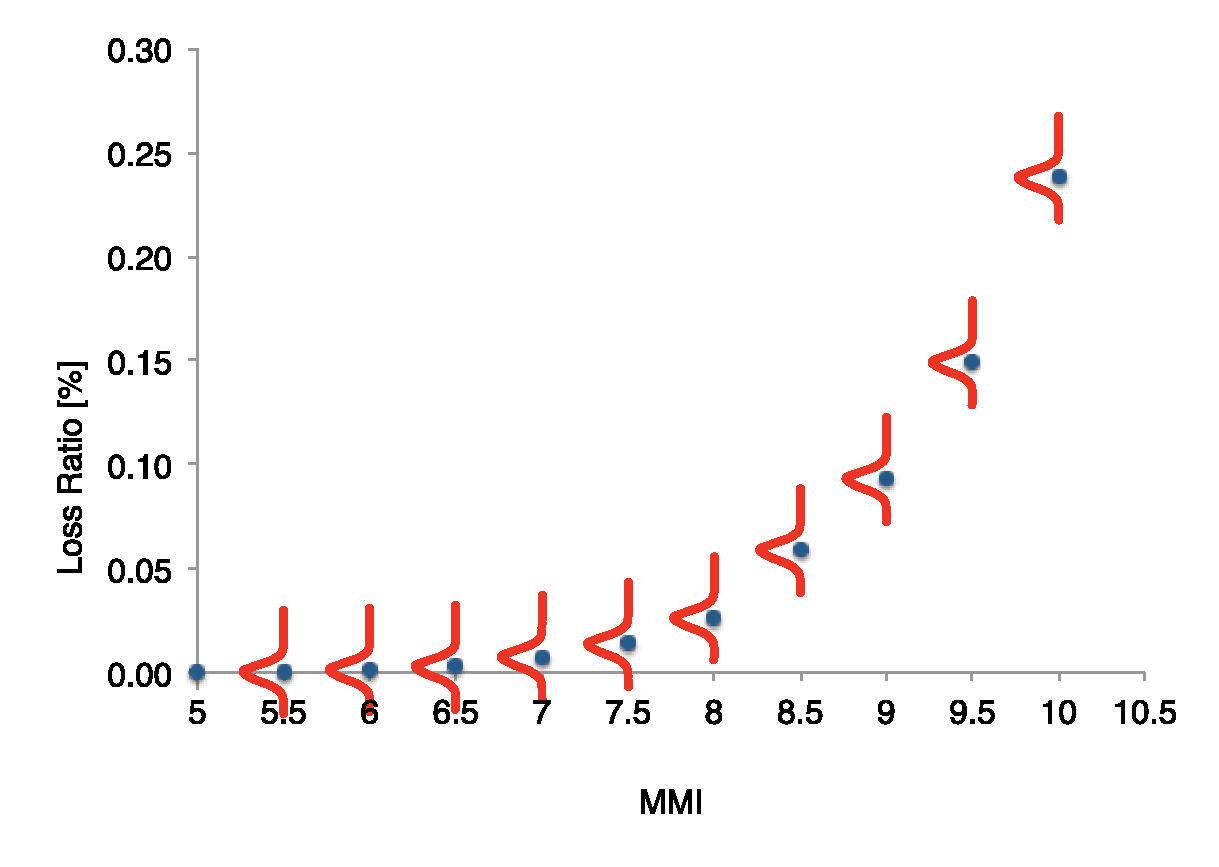
\includegraphics[width=10cm,height=6cm]{./figures/risk/VFDiscrete.eps}
\caption{Discrete vulnerability function.}
\label{fig:VFDiscrete}
\end{figure}

\color{blue}
\subsubsection{Continuous Vulnerability Functions}
\index{Physical Vulnerability!Continuous Functions}
\marginpar{Continuous vulnerability functions are not currently supported}
Continuous \glspl{vulnerability function} may be implemented in future versions of the OpenQuake engine. Continuous \glspl{vulnerability function} will probably be described by continuous distributions of mean loss ratio and other fractiles of loss ratio, with ground motion intensity. Figure \ref{fig:VFContinuous} illustrates this type of function, showing the distribution of mean loss and the 10 percent and 90 percent fractiles.

\begin{figure}[ht]
\centering
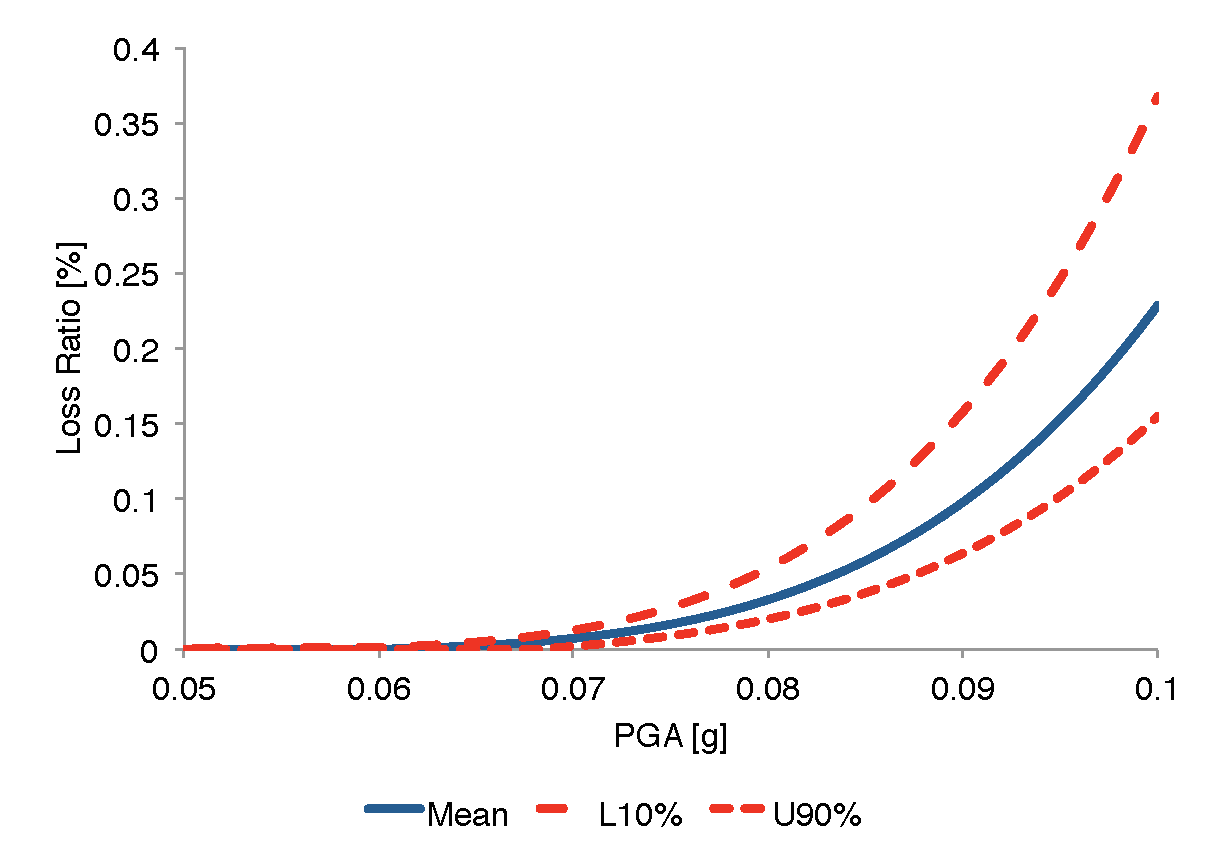
\includegraphics[width=10cm,height=6cm]{./figures/risk/VFContinuous}
\caption{Continuous vulnerability function.}
\label{fig:VFContinuous}
\end{figure}
\color{black}

\subsection{Fragility Functions}
\index{Fragility}
\Glspl{fragility function} describe the probability of exceeding a set of limit states, given an intensity measure level. When the asset category concerns structures (e.g. buildings), the intensity measure can either be structure-independent or structure-dependent. The former can be calculated directly from recorded measurements of ground shaking (e.g. peak ground acceleration, peak ground velocity, spectral acceleration at a given period of vibration, or even macroseismic intensity). The latter requires information on the characteristics of the structures in order to be calculated, for example spectral acceleration at the fundamental period of vibration, or spectral displacement at the limit state period of vibration. The calculation of these structural characteristics might be through a simple formulae (e.g. a yield period-height equation, see e.g. \citet{CrowleyPinho2004} ) or through so-called non-linear static methods, which are needed when the intensity measure is a non-linear response quantity such as spectral displacement at the limit state period of vibration (see e.g. \citet{FEMA440ATC2005}). The oq-risklib currently does not support non-linear static methods.

\subsubsection{Discrete Fragility Functions}
\index{Fragility!Discrete Functions}
\Glspl{fragility function} can be defined in a discrete way by providing, for each limit state, a list of intensity measure levels and respective probabilities of exceedance. Figure \ref{fig:FFDiscrete} presents a set of discrete \glspl{fragility function} using a macroseismic intensity measure. 

\begin{figure}[ht]
\centering
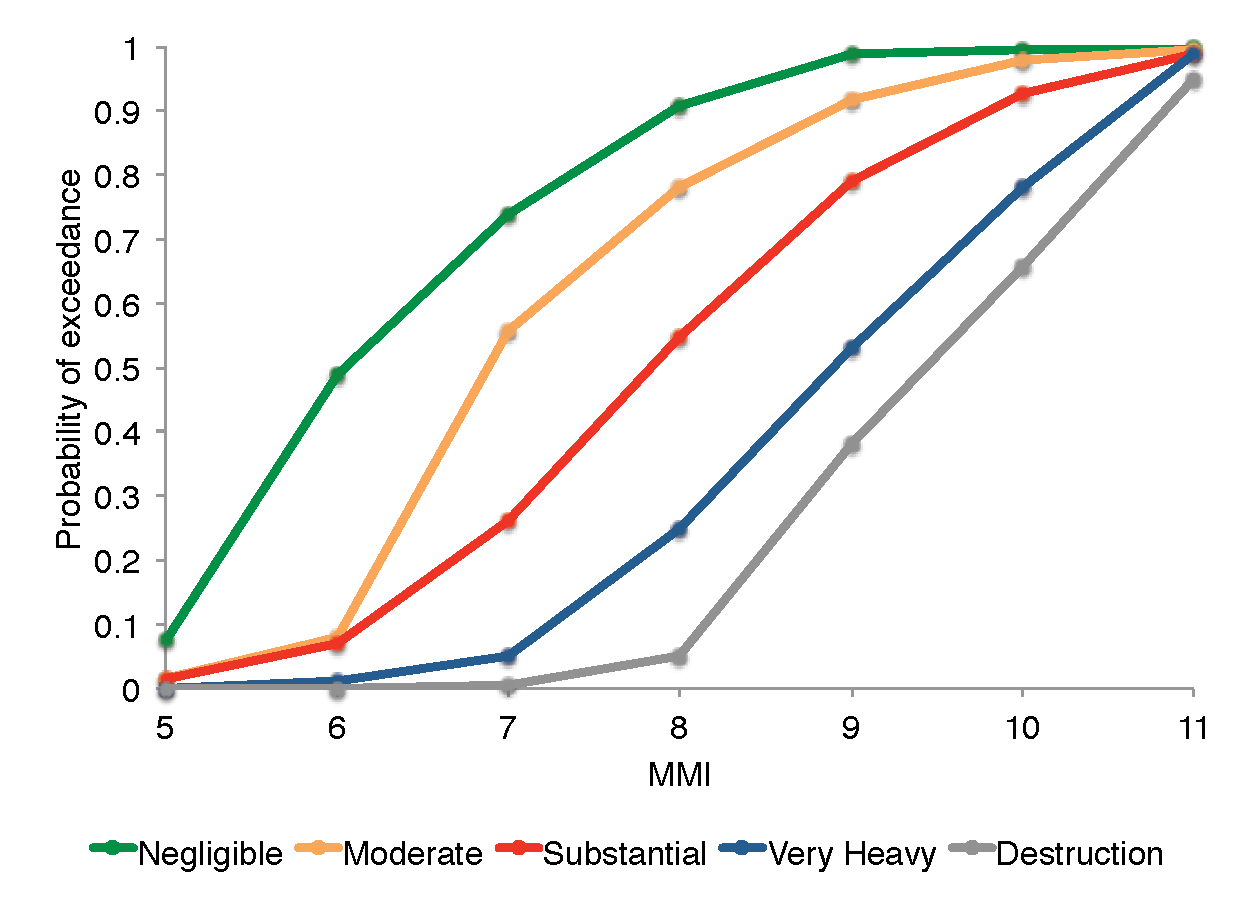
\includegraphics[width=10cm,height=6cm]{./figures/risk/FFDiscrete.eps}
\caption{Set of discrete fragility functions.}
\label{fig:FFDiscrete}
\end{figure}

\subsubsection{Continuous Fragility Functions}
\index{Fragility!Continuous Functions}
Continuous \glspl{fragility function} are defined by the parameters of a cumulative distribution function. In Figure \ref{fig:FFcontinuous} an example of a set of continuous fragility functions with a structure-dependent intensity measure is presented. 

\begin{figure}[ht]
\centering
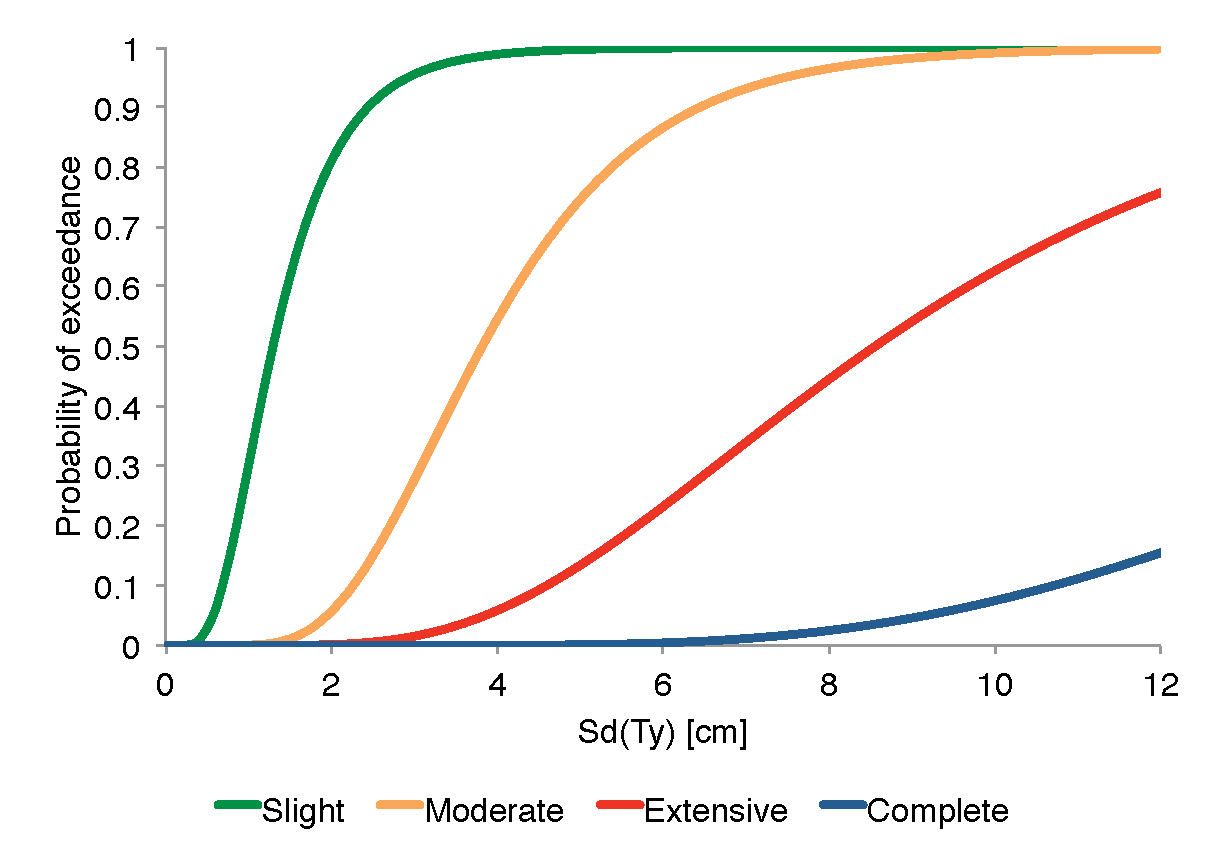
\includegraphics[width=10cm,height=6cm]{./figures/risk/FFContinuous.eps}
\caption{Set of continuous fragility functions.}
\label{fig:FFcontinuous}
\end{figure}

\color{blue}
\subsubsection{Uncertainty in Fragility Functions}
\index{Fragility!Uncertainty}
\marginpar{uncertainty in fragility functions is not currently supported}
The uncertainty in continuous glspl{fragility function} will be accounted for in future versions of the engine. Figure \ref{fig:FF_uncertainty} shows a lognormal distribution that has been fit to the data (i.e. the fragility function), and the probabilistic distribution (i.e. mean and standard deviation) to describe the uncertainty in both the logarithmic mean and logarithmic standard deviation of the fragility function. When a set of glspl{fragility function} for different limit states are used, it is also necessary to provide information on the correlation between the logarithmic means and logarithmic standard deviations of each limit state.

\begin{figure}[ht]
\centering
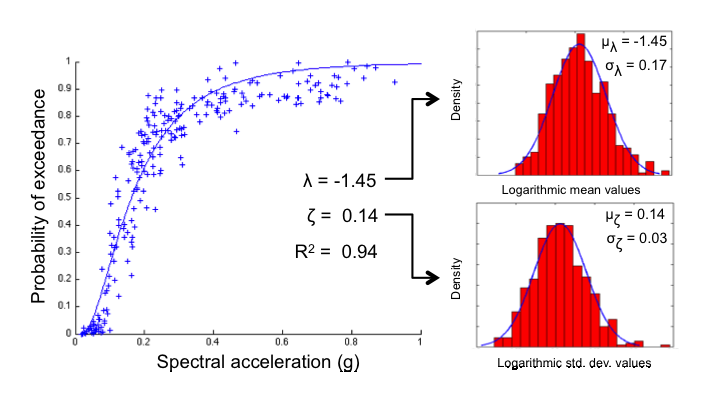
\includegraphics[width=12cm,height=6cm]{./figures/risk/FFuncertainty.eps}
\caption{Uncertainty of continuous fragility functions.}
\label{fig:FF_uncertainty}
\end{figure}


\subsection{Consequence Functions}
\index{Consequence Functions}
\marginpar{Consequence functions are not currently supported}
\Glspl{consequence function} describe the probability distribution of loss, given a performance level. For example, if the asset category is buildings and the performance level is significant damage, the \gls{consequence function} will describe the mean loss ratio, coefficient of variation and probability distribution for that level of damage. Figure \ref{fig:ConsequenceFunctions} presents the mean damage ratios for a set of performance levels proposed by two different sources. Although these functions are not directly supported, users can combine \glspl{consequence function} with \glspl{fragility function} to produce \glspl{vulnerability function} to be input into the engine.  

\begin{figure}[Ht]
\centering
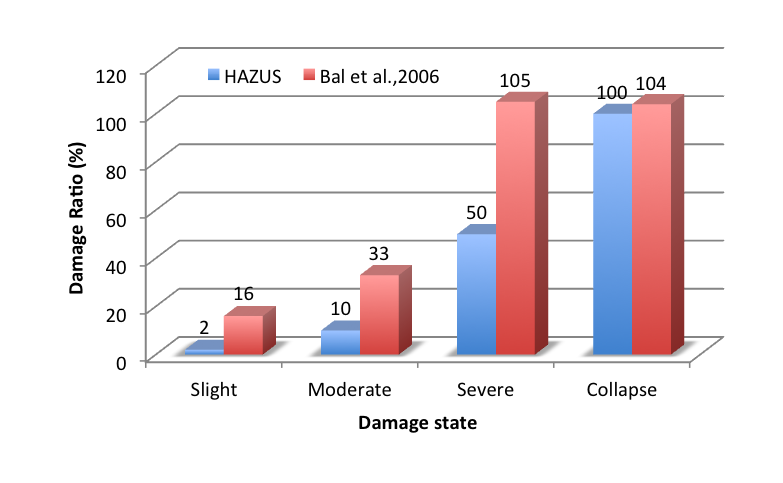
\includegraphics[width=10cm,height=6cm]{./figures/risk/ConsequenceFunction.eps}
\caption{Consequence functions adapted from  \citet{Baletal2010}}
\label{fig:ConsequenceFunctions}
\end{figure}
\color{black}

% ------------------------------------------------------------------------------
\chapter{Scenario Risk Calculator}
	\label{chap:scenario_risk}
	

\section{Introduction}
\index{Scenario Risk}
The scenario risk calculator is capable of computing losses and loss statistics from a single event for a collection of assets, given a set of \glspl{groundmotionfield}. The use of a set of \glspl{groundmotionfield} is recommended so that the aleatory variability (both inter- and intra-event) in the \gls{groundmotionpredictioneq} is modelled. The input glspl{groundmotionfield} can be calculated with oq-hazardlib or by an external software; in either case they need to be stored in the OpenQuake engine database. With the use of the oq-hazardlib, these glspl{groundmotionfield} can be calculated either with or without the spatial correlation of the ground motion residuals.

For each gls{groundmotionfield}, the intensity measure level at a given site is combined with a \gls{vulnerability function}, from which a loss ratio is randomly sampled, for each \gls{asset} contained in the \gls{exposure model}. The loss ratios that are sampled for \glspl{asset} of a given \gls{taxonomy} classification at different locations can be considered to be either independent, fully correlated, or correlated with a specific correlation coefficient. Using these results, the mean and standard deviation of the loss ratios across all \glspl{groundmotionfield} can be calculated. Loss ratios are converted into losses by multiplying by the structural value of the \gls{asset} given in the exposure model. It is furthermore possible to sum the losses throughout the region and to compute the mean and standard deviation of the total loss. 

\section{Calculation Steps}

To compute the mean loss:

\begin{enumerate}
\item For each \gls{groundmotionfield}, the intensity measure level at the location of the \gls{asset} is used to derive the mean loss ratio and associated coefficient of variation from the \gls{vulnerability function}. Since currently the \glspl{vulnerability function} are being defined in a discrete manner, it is quite probable that the intensity measure level provided by the \gls{groundmotionfield} is not contained in the \gls{vulnerability function}. In these cases, linear interpolation methods are being employed to derive the mean loss ratio at the intensity measure level of interest. 

\item The engine takes the \gls{vulnerability function} assigned to each \gls{asset} and checks if the coefficient of variation is zero. If so, the loss ratios are derived based on the mean loss ratio for each intensity measure level. Otherwise, if the uncertainty is defined, it is randomly sampled following the probabilistic distribution of the respective \gls{vulnerability function}, as described below:

\begin{equation}
\log{LR_n} = \mu + \epsilon\sigma
\end{equation}

Where $\mu$ and $\sigma$ stand for the mean and standard deviation of the logarithm of the loss ratios respectively and $\epsilon$ is a term that has a standard normal distribution with a zero mean and a standard deviation of one.  

The method used to sample epsilon depends on whether the correlation between the vulnerability uncertainty of \glspl{asset} of a given \gls{taxonomy} is to be considered or not:

\begin{itemize}

\item Perfectly correlated: the term $\epsilon$ is randomly sampled once for the first \gls{asset} and this result is used to derive the loss ratio for all the \glspl{asset} of the same \gls{taxonomy}. 

\item Correlated: the term $\epsilon$ is randomly sampled for each \gls{asset} considering the specified correlation coefficient between \glspl{asset}. 

\item Uncorrelated: the term $\epsilon$ is always randomly sampled for each \gls{asset} and therefore the correlation between the vulnerability of the \glspl{asset} is ignored.

\end{itemize}

\item The mean loss ratio for each \gls{asset} across all possible simulations of the scenario event can be calculated through the formula:

\begin{equation}
LR=\frac{\sum^m_{n=1}LR_n|IML}{m}
\end{equation}

Where $m$ stands for the number of ground motion fields simulated.

\item The mean loss can then be derived by multiplying the mean loss ratio by the value of the \gls{asset} contained in the \gls{exposure model} file.

\end{enumerate}

To compute the standard deviation of the loss:

\begin{enumerate}

\item In order to compute the uncertainty, the engine takes the set of loss ratios for each \gls{asset}, and computes the associated standard deviation using the classical formula:

\begin{equation}
SD[LR]=\sqrt{  \frac{1}{m}\sum_{n=1}^m{(LR_n-E[LR])^2} }
\end{equation}

Where $E[LR]$ stands for the mean loss ratio computed previously.

\item The standard deviation of the absolute loss can finally be computed by multiplying the standard deviation of the loss ratio by the value of the respective \gls{asset}.

\end{enumerate}

\section{Calculator Output}
The output of the Scenario Risk Calculator currently comprises loss statistics (mean total loss and standard deviation of total loss) and loss maps. Loss maps are comprised by a set of loss nodes, which are associated with a pair of coordinates. For each node, one or more loss values might exist, due to the fact that several different \glspl{asset} can be located at the same location.  Figure \ref{fig:detlosses} presents an example of a loss map containing the expected economic losses for residental buildings located in Nepal, considering a rupture of magnitude 7.0Mw in the central part of the country.

\begin{figure}[ht]
\centering
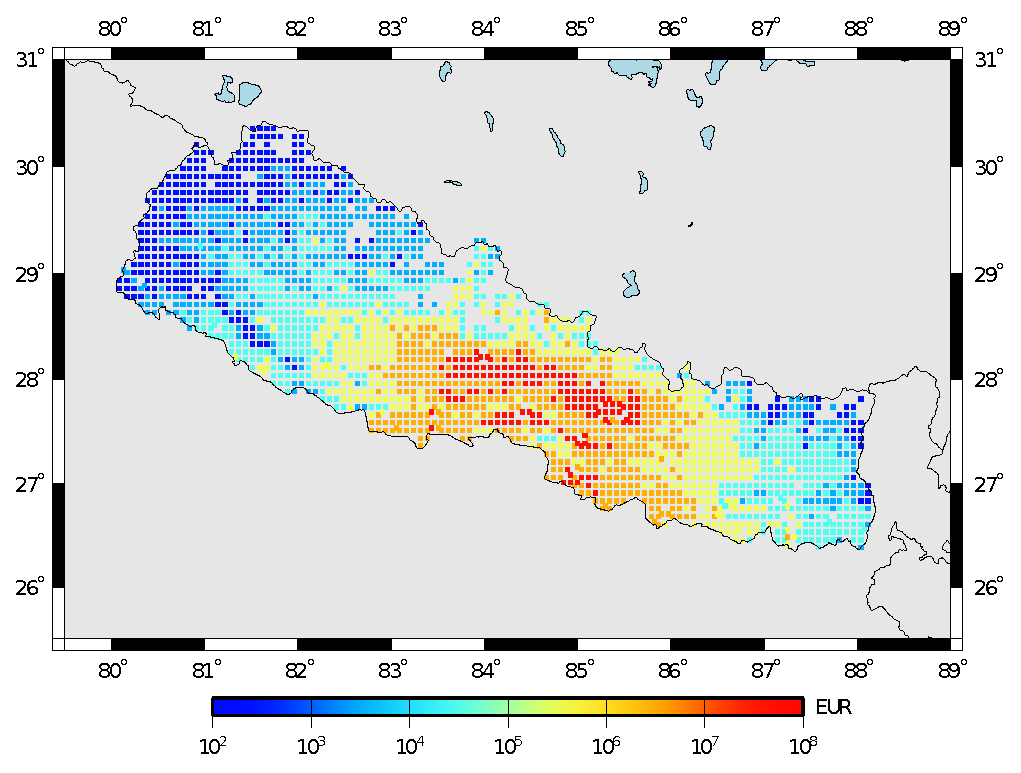
\includegraphics[width=12cm,height=7cm]{./figures/risk/LossmapDet.eps}
\caption{Loss map with the distribution of mean economic losses for residential buildings in Nepal.}
\label{fig:detlosses}
\end{figure} 
% ------------------------------------------------------------------------------
\chapter{Scenario Damage Calculator}
	\label{chap:scenario_damage}
	

\section{Introduction}
\index{Scenario Damage}
The scenario damage calculator can be employed to estimate the distribution of damage due to a single earthquake, for a spatially distribute building portfolio. Similarly to what has been described for the scenario risk calculator, a finite \gls{rupture} should be used to derive sets of \glspl{groundmotionfield}. 

In this calculator, each \gls{groundmotionfield} is combined with a \gls{fragility model} (discrete or continuous), in order to compute the fractions of buildings in each damage state. These fractions are calculated based on the difference in probabilities of exceedance between consecutive limit state curves at a given intensity measure level. This process is repeated for each \gls{groundmotionfield}, leading to a list of fractions for each \gls{asset}. These results can then be multiplied by the respective number or area of buildings in order to obtain the absolute building damage distribution.

\section{Calculation Steps}

\begin{enumerate}
\item For each \gls{groundmotionfield}, the intensity measure level at the location of the \gls{asset} is used to derive the
fraction of buildings in each damage state. In order to do so, the distance between each pair of consecutive limit states is calculated. This process is illustrated in Figure \ref{fig:FragilityProcess}, using a continuous \gls{fragility function}.

\begin{figure}[ht]
\centering
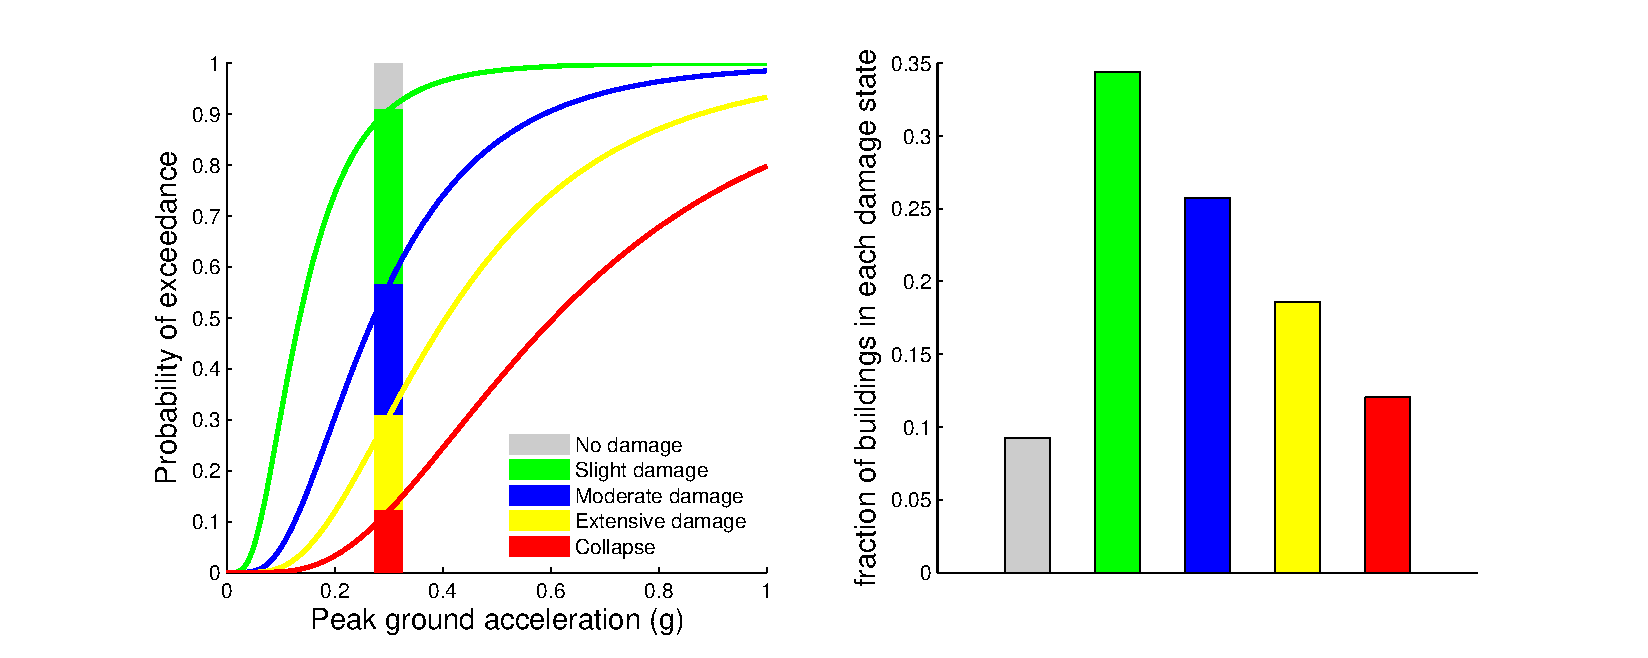
\includegraphics[width=14cm,height=5cm]{./figures/risk/Fragility_process.eps}
\caption{Representation of the fractions of building in each damage states, for a given intensity measure level (0.3 g).}
\label{fig:FragilityProcess}
\end{figure}

When a continuous \gls{fragility function} is used for the calculations, the fractions of building in each damage state are calculated using the analytical expression of the lognormal cumulative distribution functions. On the other hand, if a discrete \gls{fragility function} was chosen, these fractions are computed using linear interpolation between the pair of points either side of the intensity measure level.

\item Step 1 is repeated for each \gls{groundmotionfield}, leading to a list of fractions (one per damage state), for each \gls{asset}. From this list of values, the mean ($E[FR]$) and standard deviation ($SD[FR]$) for each fraction can be estimated using the following formulae:

\begin{equation}
E[FR]=\frac{\sum^m_{n=1}FR_n|IML}{m}
\end{equation}

\begin{equation}
SD[FR]=\sqrt{  \frac{1}{m}\sum_{n=1}^m{(FR_n-E[FR])^2} }
\end{equation}
 
Where $m$ stands for the number of \glspl{groundmotionfield} simulated. 

\item These fractions of buildings in each damage state can be multiplied by the quantity of the respective asset, leading to the mean and standard deviation of the number or area of buildings in each damage state (see Figure \ref{fig:AssetDis}). 

\item This calculator is also capable of estimating the aggregated number or area of buildings from the same \gls{taxonomy} in each damage state (see Figure \ref{fig:TaxDis}). In order to do so, for each \gls{groundmotionfield}, the absolute quantity of buildings in each damage state is calculated, and aggregated according to their \gls{taxonomy}. After processing all the \glspl{groundmotionfield}, the associated statistics for each building \gls{taxonomy} are calculated according to the formulae described in Step 2.

\item The total damage distribution is also calculated, by summing the quantity of buildings in each damage state, across all the \glspl{asset} existing in the building portfolio. This calculation will lead to a single damage distribution, represented by a mean and standard deviation for each damage state (see Figure \ref{fig:TotalDis}).

\end{enumerate}

\section{Calculator Output}
The output of the Scenario Damage Calculator currently comprises damage distributions at three levels: per \gls{asset}, per building \gls{taxonomy} and total. In addition, with this calculator, is it also possible to extract collapse maps, which contain the spatial distribution of the number or area of collapsed buildings throughout the region of interest (see Figure \ref{fig:CollapseMap}). In the figures shown herein, examples of the outputs are depicted for a scenario event of magnitude 7.0Mw in the central region of Nepal.

\begin{figure}[ht]
\centering
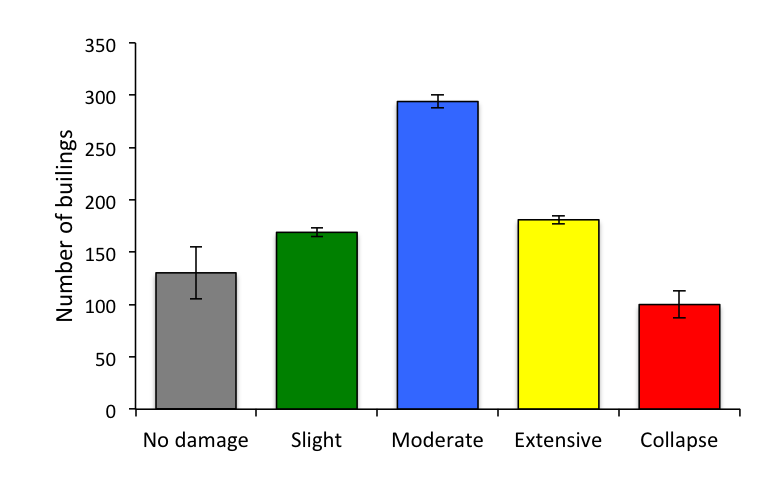
\includegraphics[width=8cm,height=5cm]{./figures/risk/AssetDisaggregation.eps}
\caption{Damage distribution for a single asset.}
\label{fig:AssetDis}
\end{figure} 

\begin{figure}[ht]
\centering
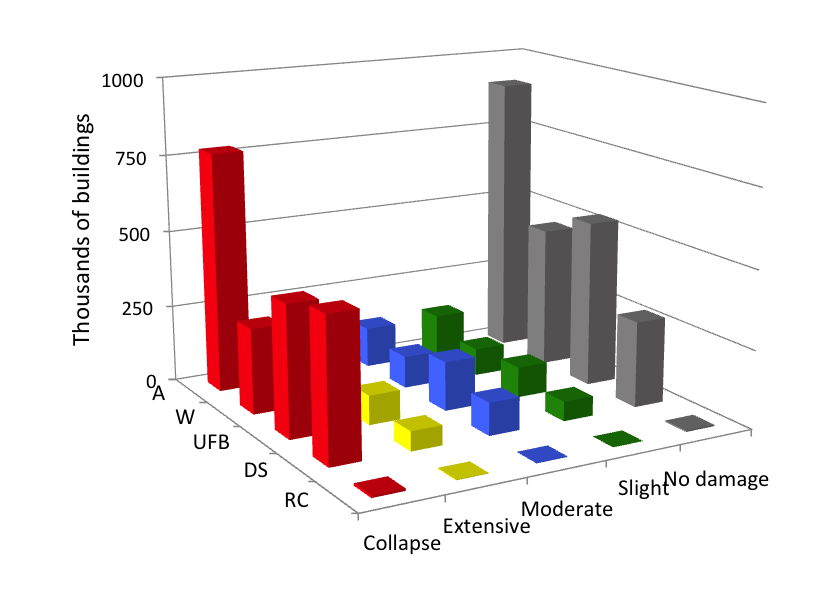
\includegraphics[width=8cm,height=5cm]{./figures/risk/TaxonomyDisaggregation.eps}
\caption{Damage distribution according to the building taxonomy.}
\label{fig:TaxDis}
\end{figure} 

\begin{figure}[ht]
\centering
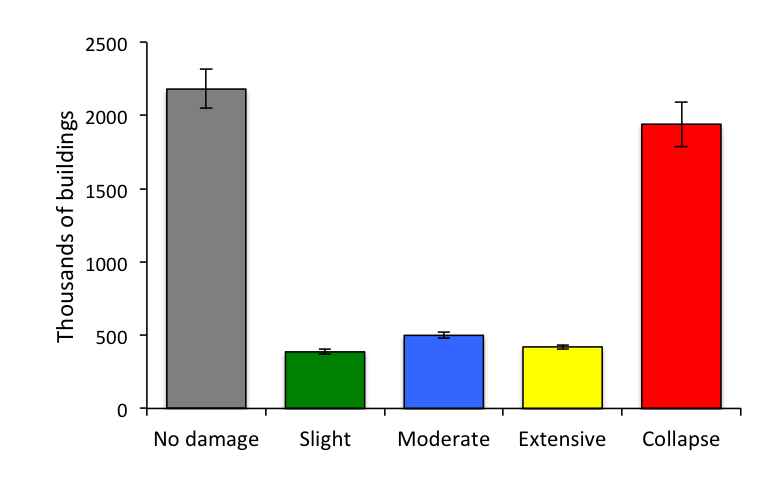
\includegraphics[width=8cm,height=5cm]{./figures/risk/TotalDis.eps}
\caption{Damage distribution of the whole building portfolio.}
\label{fig:TotalDis}
\end{figure} 

\begin{figure}[ht]
\centering
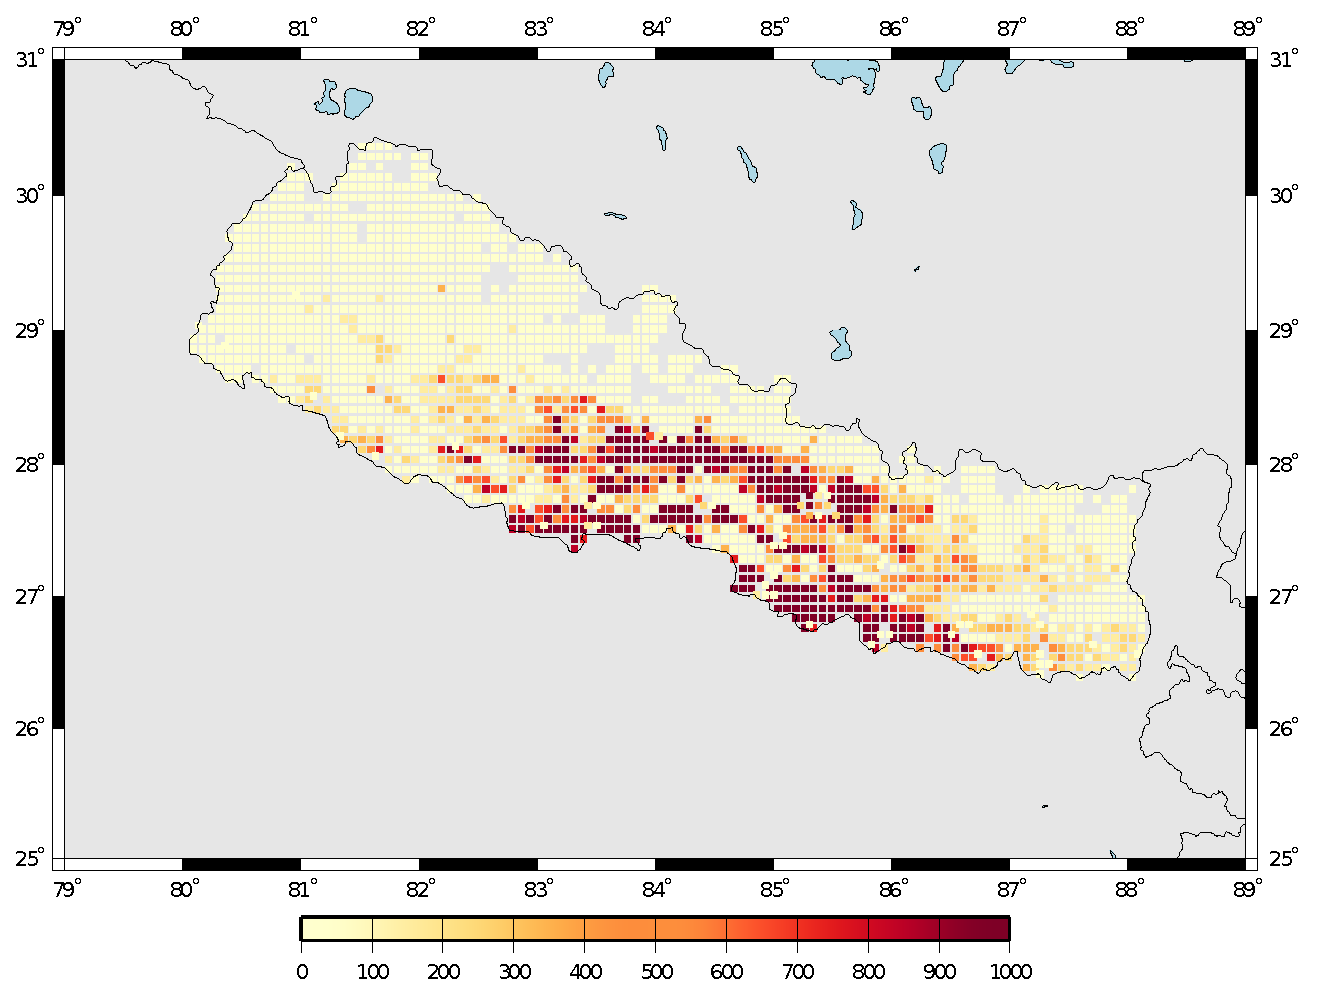
\includegraphics[width=12cm,height=7cm]{./figures/risk/CollapseMap.eps}
\caption{Collapse map considering the whole building portfolio.}
\label{fig:CollapseMap}
\end{figure} 
% ------------------------------------------------------------------------------
\chapter{Probabilistic Event-Based Risk Calculator}
	\label{chap:risk_prob_event_based}
	\section{Introduction}
\index{Probabilistic Risk!Event-Based}
The probabilistic event-based risk calculator uses \glspl{stochasticeventset} and associated \glspl{groundmotionfield} to compute loss exceedance curves for each \gls{asset} contained in an \gls{exposure model}. This calculator thus requires \glspl{groundmotionfield} from a number of stochastic events as an input, which the engine can calculate using the oq-hazardlib.

For each \glspl{groundmotionfield}, the intensity measure level at a given site is combined with a \gls{vulnerability function}, from which a loss ratio is randomly sampled, for each \gls{asset} contained in the \gls{exposure model}. The loss ratios that are sampled for \glspl{asset} of a given \gls{taxonomy} classification at different locations are considered to be either independent or correlated. The losses for a given asset are calculated using all of the \glspl{groundmotionfield}, leading to list of events and associated loss ratios. This list is then sorted from the highest loss ratio to the lowest. The rate of exceedance of each loss ratio is calculated by dividing the number of exceedances of that loss ratio by the number of \glspl{stochasticeventset} multiplied by the length of each event set. By assuming a Poissionian distribution of the occurrence model, the probability of exceedance of each loss ratio is calculated. If a total loss curve for a portfolio of \glspl{asset} is required, a secondary module is used in order to sum the losses from all the \glspl{asset} in the exposure file, per event, before calculating the exceedance distribution of loss. This distribution of the total losses per event can also be extracted, and it is termed here as an \gls{eventLossTable}.

Similarly to what has been described for the Scenario Risk Calculator (see section \ref{chap:scenario_risk}), this module can compute \gls{insuredLosses} following the same approach (i.e. modifying the  loss based on the \gls{deductible} and \gls{limit} for each cost type).

This calculator is also capable of performing \gls{lossdisaggregation} in terms of magnitude/distance or latitude/longitude. In order to do so, the losses at each location are disaggregated based on the aforementioned parameters, and a loss percentage for each possible combination is calculated.

\section{Calculation Steps}

To compute the loss exceedance curves:

\begin{enumerate}
\item The oq-engine starts by using the set of \glspl{groundmotionfield} to extract the intensity measure levels for the location of each \gls{asset}. 
 
\item Then the oq-engine takes the \gls{vulnerability function} assigned to each \gls{asset} and checks if the coefficient of variation is zero. If so, the loss ratios are derived based on the mean loss ratio for each intensity measure level. Otherwise, if the uncertainty is defined, it is randomly sampled following the probabilistic distribution, mean loss ratio and associated coefficient of variation of the respective function, as described below:

\begin{equation}
\log{LR_n} = \mu + \epsilon\sigma
\end{equation}

Where $\mu$ and $\sigma$ stand for the mean and standard deviation of the logarithm of the loss ratios respectively and $\epsilon$ is a term that has a standard normal distribution with a zero mean and a standard deviation of one.  

The method used to sample epsilon can follow tree approaches depending on whether the correlation between the vulnerability of \glspl{asset} of a given \gls{taxonomy} is to be considered or not:

\begin{itemize}

\item Perfectly correlated: the term $\epsilon$ is randomly sampled once for the first \gls{asset} and this result is used to derive the loss ratio for all the \glspl{asset} of the same \gls{taxonomy}. 

\item Correlated: the term $\epsilon$ is randomly sampled for each \gls{asset} considering the specified correlation coefficient between \glspl{asset}. 

\item Uncorrelated: the term $\epsilon$ is always randomly sampled for each \gls{asset} and therefore the correlation between the vulnerability of the \glspl{asset} is ignored.
\end{itemize}

\item Each loss ratio is multiplied by the associated asset value, leading to the absolute loss values. If these losses are related with the structural, non-structural or contents cost, the \gls{insuredLosses} module can be used to modify the \gls{groundupLosses} according to the associated \gls{deductible} and \gls{limit} thresholds, as described in section \ref{chap:scenario_risk}.

\item In this method the losses to each \gls{asset} for each event are estimated and then sorted from highest to lowest. The rate of exceedance of each loss is calculated by dividing the number of exceedances of that loss by the number of \glspl{stochasticeventset} multiplied by the length of each event set. Hence, the top loss will have zero exceedances, the next loss ratio will have one exceedance, and so on.

The following formula is employed to compute the rate of exceedance:

\begin{equation}
\lambda(L_n) = \frac{NE_{L}}{TSES}
\end{equation}

Where  $\lambda$ stands for the rate of exceedance of the respective loss ratio, $NE_{L}$ stands for the number of exceedances of the given loss, and $TSES$ stands for the time span of all \glspl{stochasticeventset}, i.e. the number of \glspl{stochasticeventset} multiplied by the time span of each.

\item Assuming a Poissonion distribution of the occurrence model, the probability of exceedance of the set of losses in a given time span can be derived using the following formula:

\begin{equation}
PE(L_n) = 1-\exp{-\lambda_n\times t}
\end{equation}

Where $t$ stands for the time span used to produce the \gls{stochasticeventset}.

\end{enumerate}

To perform the loss disaggregation:

\begin{enumerate}

\item For the disaggregation of the losses it is necessary to provide the coordinates of the locations where this procedure should be employed. Then, for the selected locations, the oq-engine calculates the sum of the losses (considering all the assets existing at each of the selected sites) for each seismic event. In addition, the rupture distance (Joyner-Boore) and coordinates of the point within the vertical projection of the rupture plane closest to each site are estimated. An example of this type of information is presented in Figure \ref{fig:SetLosses}, for 20 stochastically produced seismic events.

\begin{figure}[ht]
\centering
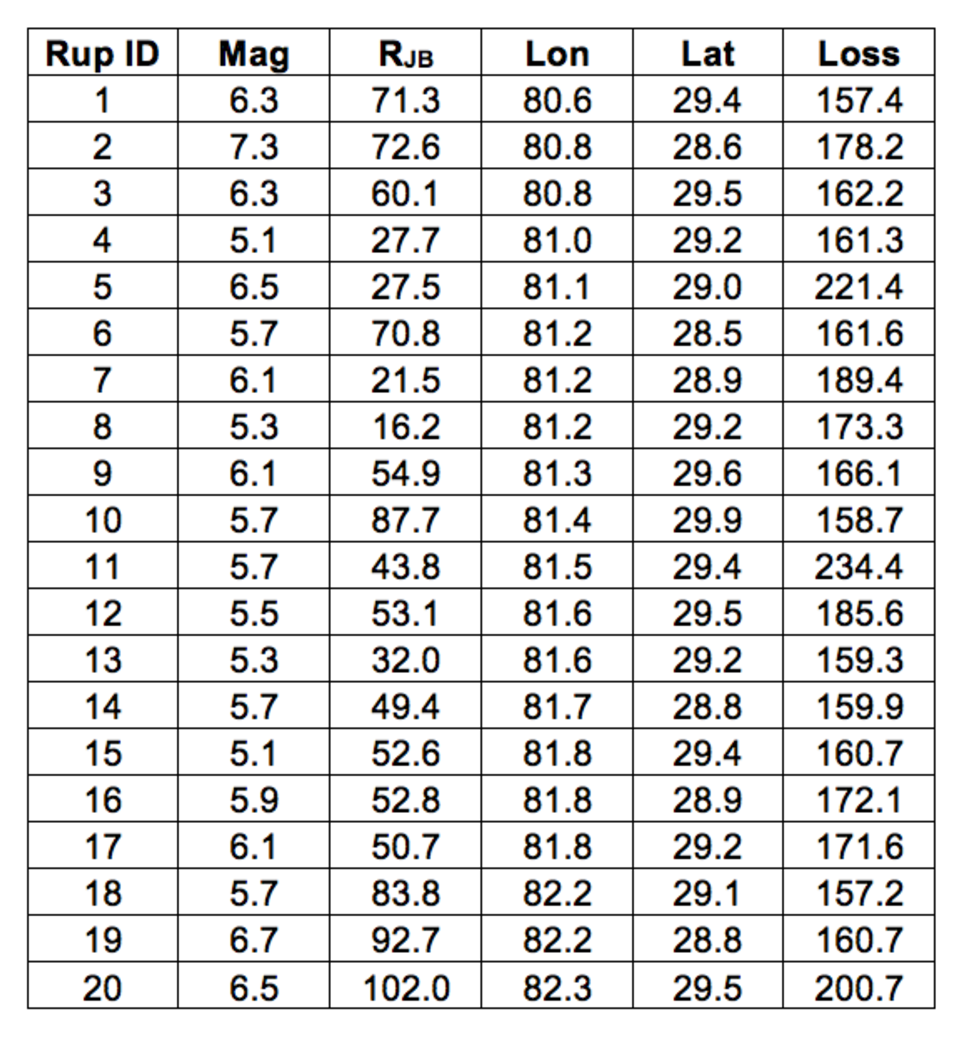
\includegraphics[width=9cm,height=10cm]{./figures/risk/SetLosses.eps} 
\caption{Economic losses from a single asset for a set of seismic events.}
\label{fig:SetLosses}
\end{figure} 

\item The oq-engine calculates the range (maximum and minimum values) of the list of magnitudes, distances, latitudes and longitudes across all the events, and using the increment defined for each parameter, a set of linearly spaced bins is calculated. Then, the losses from every seismic event are aggregated depending into which combination of magnitude/distance or latitude/longitude they fall. The previously presented losses have been disaggregated according to these two combinations as presented in Figure \ref{fig:Dis}:

\begin{figure}[ht]
\centering
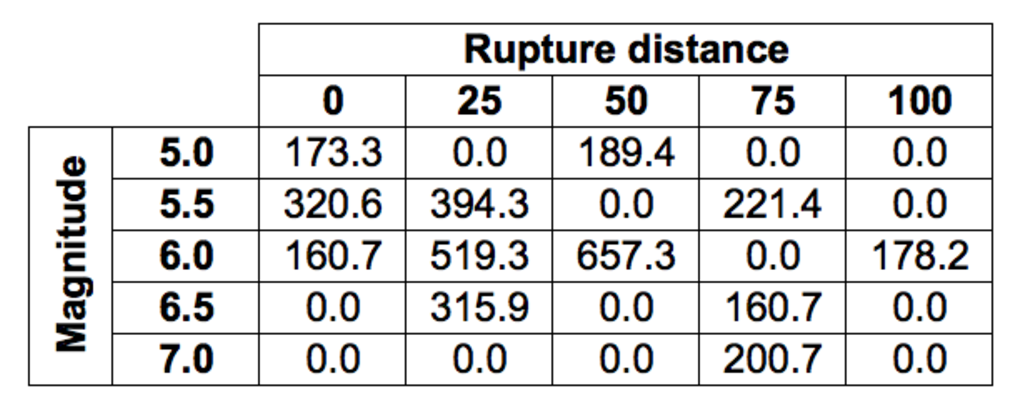
\includegraphics[width=8cm,height=3cm]{./figures/risk/DisaggregationDistMag.eps} 
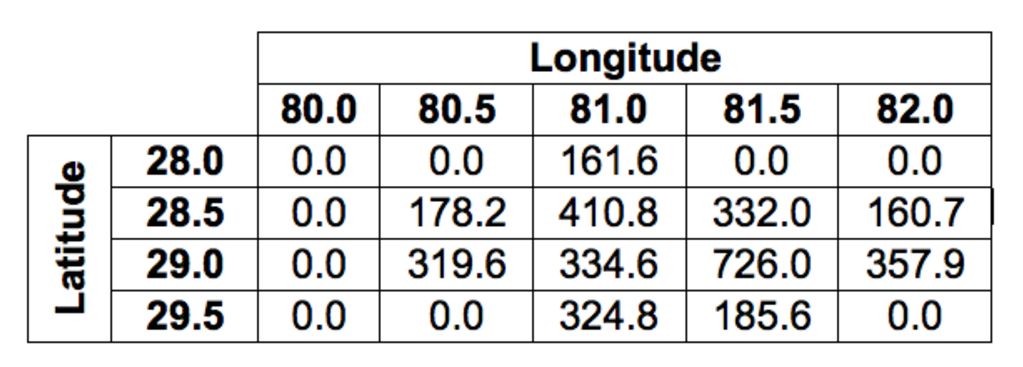
\includegraphics[width=8cm,height=2.8cm]{./figures/risk/DisaggregationCoor.eps} 
\caption{Disaggregation of the economic losses according to a set of magnitude/distance and latitude/longitude combinations.}
\label{fig:Dis}
\end{figure} 

\item The resulting losses for each pair of parameters (magnitude/distance and latitude/longitude) are divided by the total loss across all the events. This percentage of the overall loss for each combination is depicted in Figure \ref{fig:disaggregation} in the following section.
\end{enumerate}

\section{Calculator Output}
The output of this calculator comprises loss exceedance curves and loss maps. Loss exceedance curves are represented by a list of losses and respective probabilities of exceedance. Furthermore, each curve is associated with a pair of coordinates, an end branch label (that allows the curve to be connected to the set of specifications used in the calculations) and an asset ID (that permits tracking of the asset that each loss curve was computed for). Loss maps for a given probability of exceedance in a given time span can be produced, as well as maps of mean loss within a given time span. Figure \ref{fig:LossCurve01} and \ref{fig:LossCurve001} present a loss map for a probability of exceedance of 1\% and 10\% in 50 years for residential buildings located in Nepal, respectively. 

\begin{figure}[H]
\centering
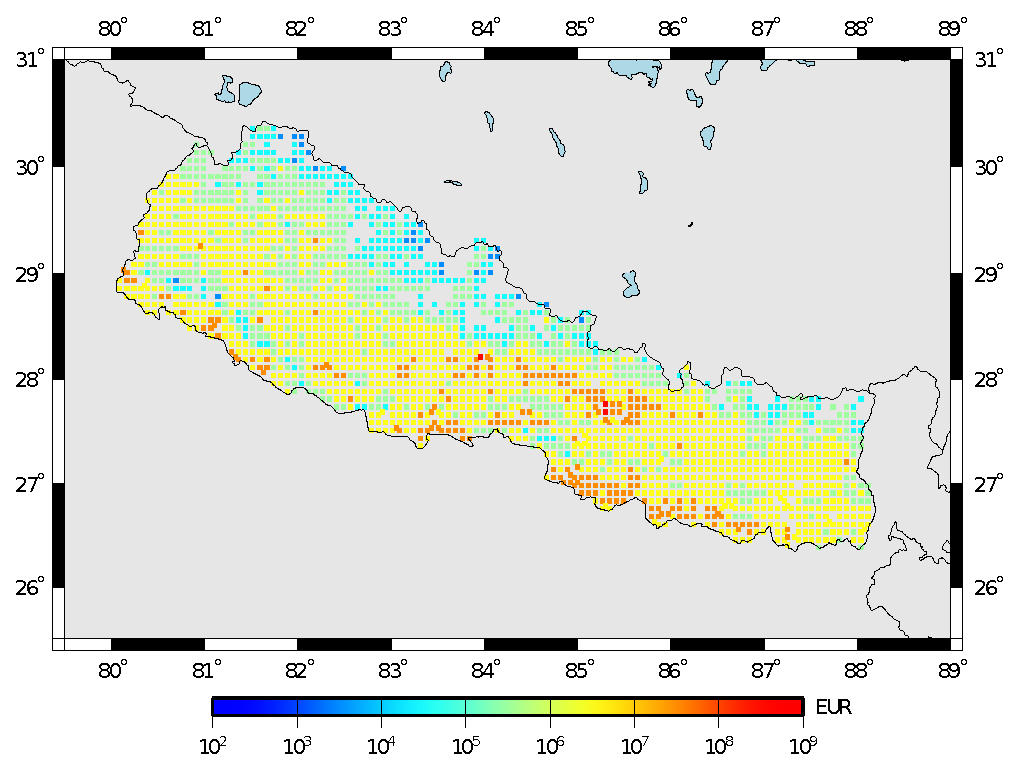
\includegraphics[width=12cm,height=8cm]{./figures/risk/LossMap01.eps} 
\caption{Loss map for a probability of exceedance of 10\% in 50 years.}
\label{fig:LossCurve001}
\end{figure} 

\begin{figure}[H]
\centering
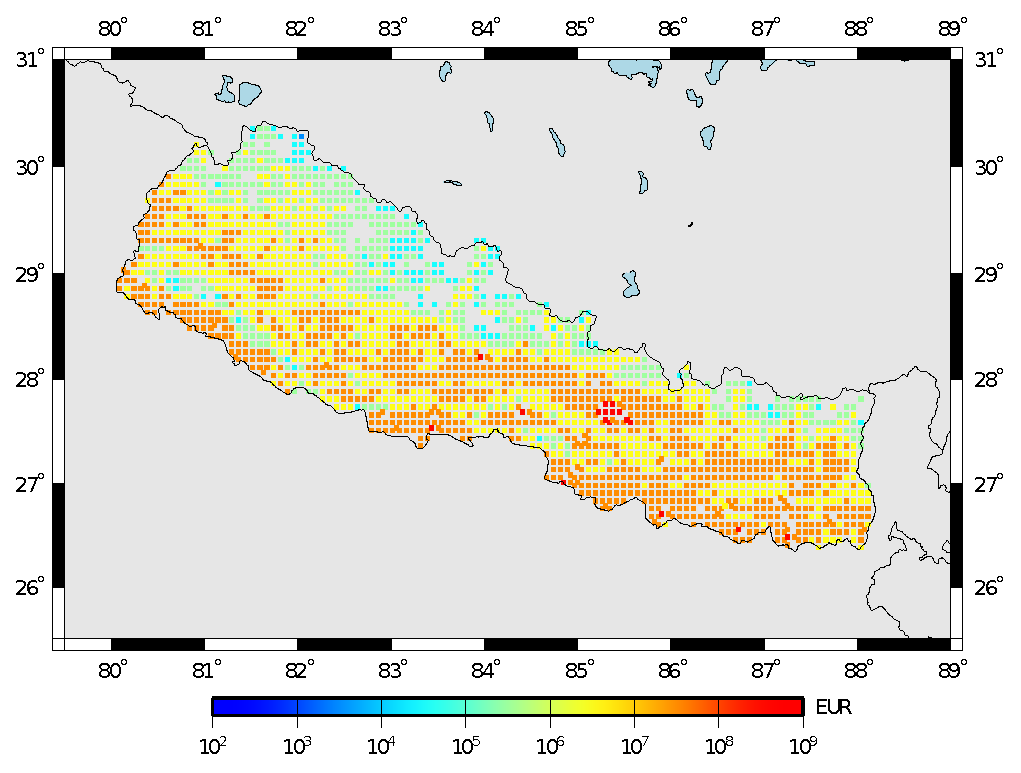
\includegraphics[width=12cm,height=8cm]{./figures/risk/LossMap001.eps} 
\caption{Loss map for a probability of exceedance of 1\% in 50 years.}
\label{fig:LossCurve01}
\end{figure} 

For this calculator, total loss exceedance curves can be produced which combine the losses to all \glspl{asset} per event. It is noted that loss exceedance curves which present the probability of exceedance of the aggregate annual losses, or maximum annual losses, are not yet supported in the oq-risklib. In Figure \ref{fig:ProbLosses}, a total loss exceedance curve for the residential building portfolio in Nepal is presented. 
 
\begin{figure}[H!]
\centering
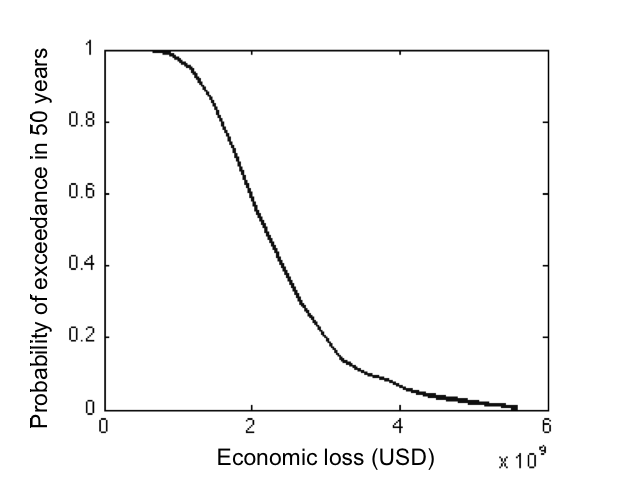
\includegraphics[width=8cm,height=6cm]{./figures/risk/LossCurveIstanbul.eps}
\caption{Total loss exceedance curve for RC buildings.}
\label{fig:ProbLosses}
\end{figure} 

For what concerns the \glspl{eventLossTable}, the oq-engine can extract the total loss across all the assets for each seismic event. The results is a table with the rupture id, magnitude and total loss, as illustrated in Figure \ref{fig:eventLossTable}.

\begin{figure}[H!]
\centering
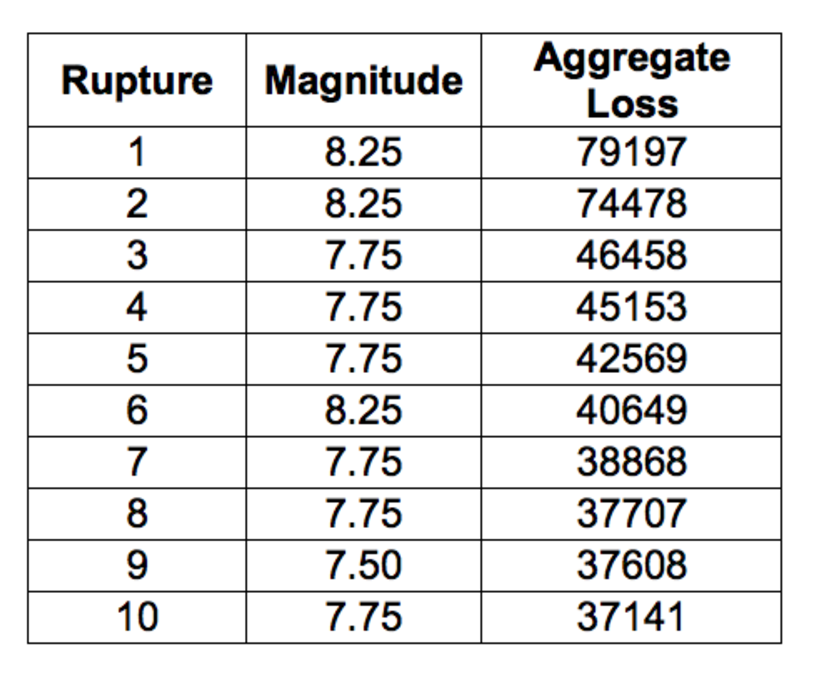
\includegraphics[width=6cm,height=5cm]{./figures/risk/EventLossTable.eps}
\caption{Example of an \gls{eventLossTable}.}
\label{fig:eventLossTable}
\end{figure} 

The output of the \gls{lossdisaggregation} is composed by the loss fraction associated to each combination of parameters (magnitude/distance or latitude/longitude), as presented in Figure \ref{fig:disaggregation} .

\begin{figure}[H!]
\centering
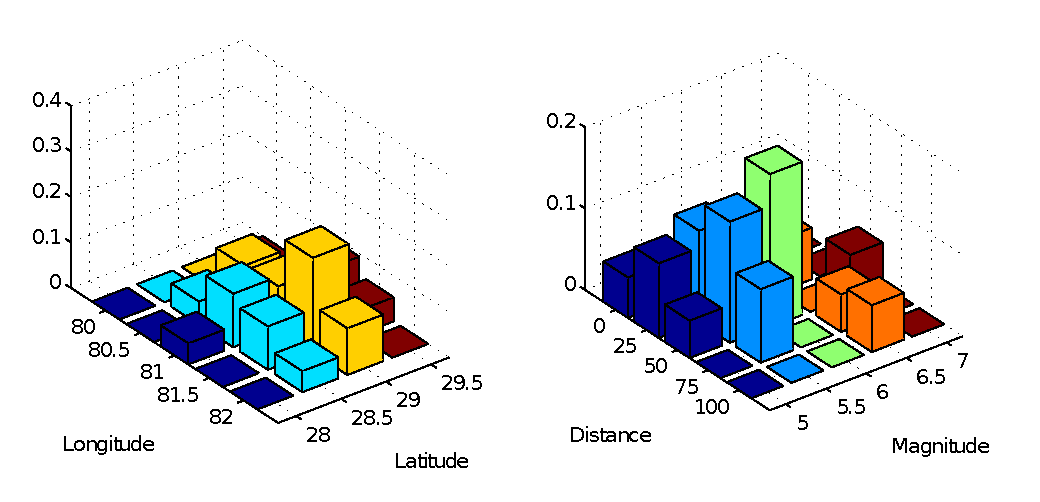
\includegraphics[width=14cm,height=6.5cm]{./figures/risk/Disaggregation.eps}
\caption{Example of a loss disaggregation according to a set of magnitude/distance and latitude/longitude combinations.}
\label{fig:disaggregation}
\end{figure} 

% ------------------------------------------------------------------------------
\chapter{Classical PSHA-Based Risk Calculator}
	\label{chap:risk_psha_based}
	\section{Introduction}
\index{Probabilistic Risk!PSHA-based}
The classical PSHA-based risk calculator can be used to calculate loss exceedance curves for single \glspl{asset}, calculated site by site, using hazard curves. This calculator thus requires hazard curves as an input, which the engine can calculate using the oq-hazardlib. Currently, this calculator is only capable of computing ground-up losses, thought insured losses will be covered in future releases.

\section{Calculation Steps}

\begin{enumerate}

\item By default, the oq-hazardlib computes hazard curves for a set of intensity measure levels that are pre-defined in the configuration file. If the user wishes to use oq-hazardlib to compute the hazard for the risk calculations, then a feature can be used which reads the \gls{vulnerability model} and uses the intensity measure levels (IMLs) defined therein when producing the hazard curve. If instead externally produced hazard curves are used, the user needs to ensure that the IMLs in the hazard curves cover the full range required by the \glspl{vulnerability function}. 

\item To use this calculator, the hazard curves need first to be converted into probability mass functions (e.g. probability of occurrence of a discrete set of intensity measure levels). To do so, the engine starts by reading the intensity measure levels from the discrete \glspl{vulnerability function}, and computes the central value between consecutive levels. Two consecutive values define the boundaries of the interval for each intensity measure level and by relating these limits with the hazard curve, the engine computes the corresponding probabilities of exceedance. Figure \ref{fig:ProbOccurrence} contains a discrete \gls{vulnerability function} (bottom figure) and a hazard curve (top figure) in which the definition of the interval for a given intensity measure level and associated estimation of the probabilities of exceedance of each limit are illustrated. 

\begin{figure}[ht]
\centering
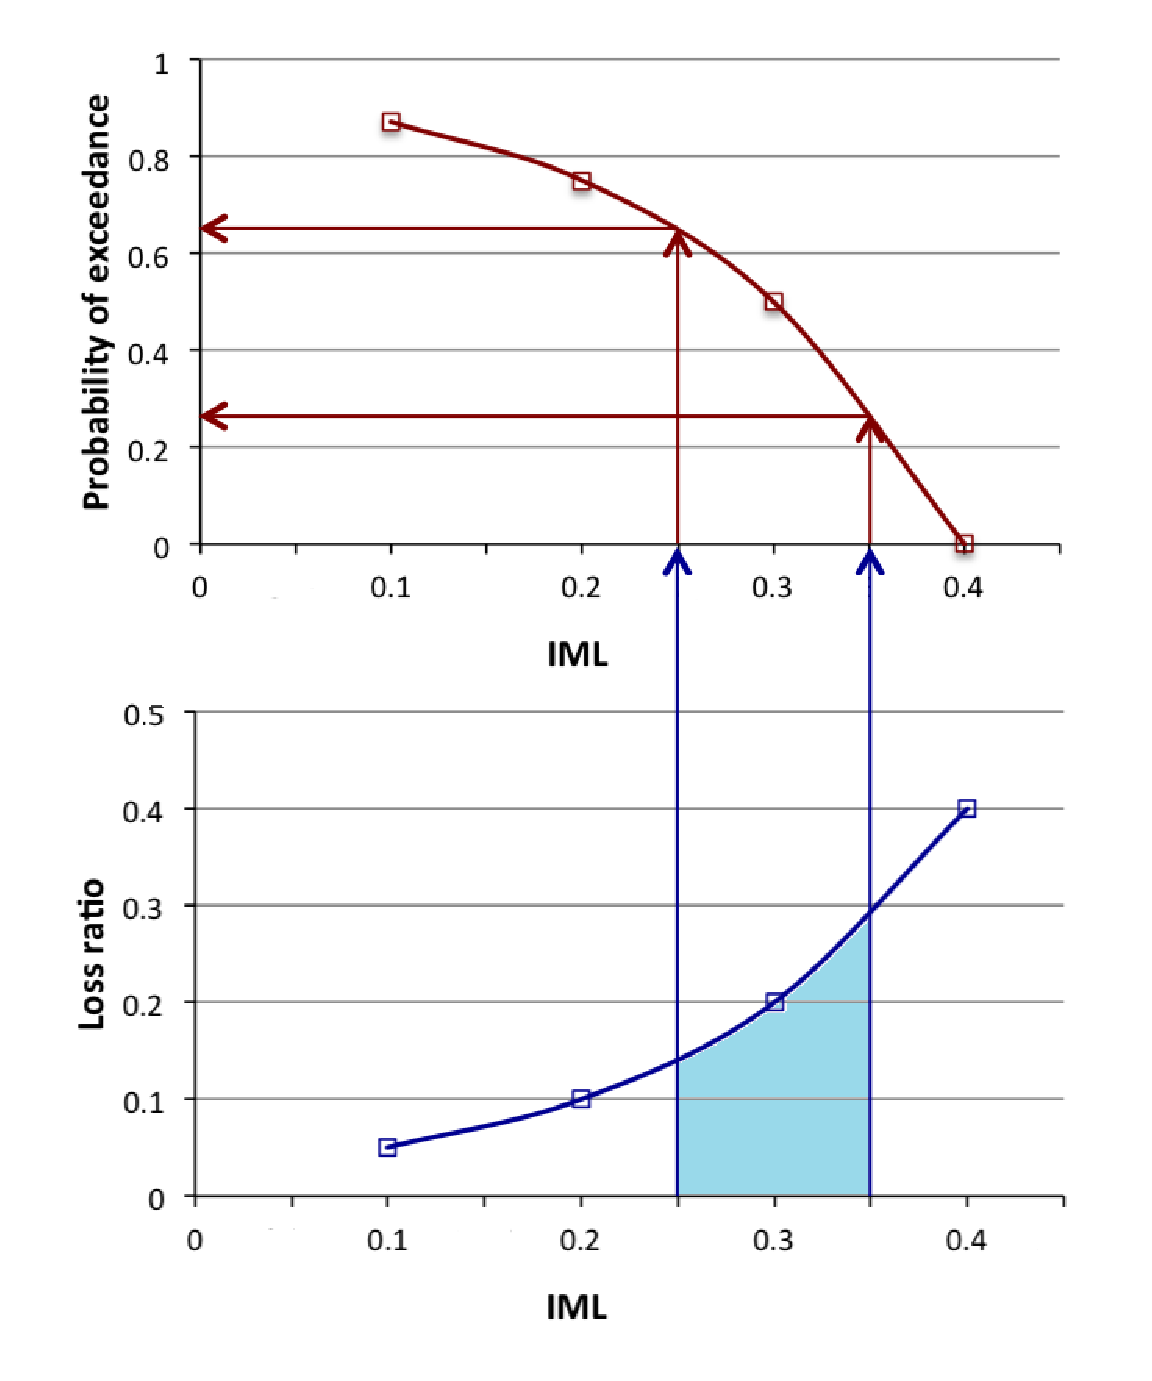
\includegraphics[width=6.5cm,height=7cm]{./figures/risk/ProbOccurrence.eps}
\caption{Workflow to estimate the probabilities of exceedance of the boundaries of each intensity measure level.}
\label{fig:ProbOccurrence}
\end{figure}

\item The probability of occurrence of the intensity measure levels that fall within each interval can be derived by subtracting the probabilities of exceedance of the lower and upper limits, as described by the following formula:

\begin{equation}
PO= PE[lower bound]-PE[upper bound]
\end{equation}

\item The discrete \glspl{vulnerability function} for each \gls{asset} are converted into loss ratio exceedance matrices (e.g. matrices which describe the probability of exceedance of each loss ratio for a discrete set of intensity measure levels). These matrices have a number of columns equal to the number of intensity measure levels defined on the \gls{vulnerability function} and a number of rows that can go from the number of loss ratios defined by the discrete function, up to any multiple of this number. In order to properly incorporate the probabilistic distribution of loss ratios per intensity measure level, the probabilities of exceedance should be computed not just for the loss ratios defined on the \gls{vulnerability function}, but also for many intermediate values between consecutive loss ratios. Following a number of sensitivity analyses, it appears that 5 intermediate values between consecutive loss ratios is a reasonable value, however, this is a parameter that can be adjusted by the user. Figure \ref{fig:LREM} contains an example of a discrete \gls{vulnerability function} and the respective loss ratio exceedance matrix (in light grey).

\begin{figure}[htb]
\centering
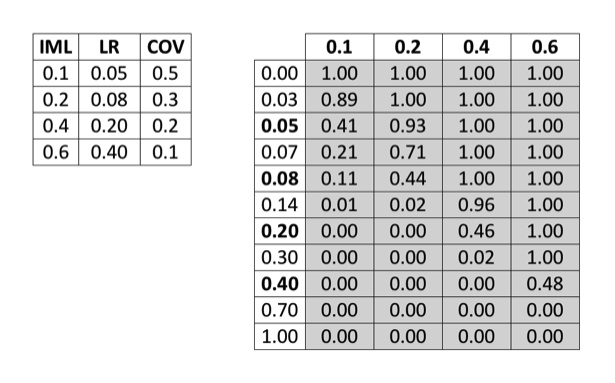
\includegraphics[width=9cm,height=5.5cm]{./figures/risk/LREM.eps}
\caption{Example of a discrete vulnerability function and respective loss ratio exceedance matrix.}
\label{fig:LREM}
\end{figure}

Note that for this example only one intermediate value was considered between consecutive loss ratios and in order to consider the whole distribution of the loss ratios, the matrix was computed considering a minimum and maximum loss ratio of 0 and 1 respectively.

\item Finally, each column of the aforementioned matrix is multiplied by the probability of occurrence of the respective intensity measure level (extracted from the hazard curves) to produce a conditional loss ratio exceedance matrix.  Then, for each loss ratio the probabilities of exceedance are summed, leading to a loss ratio exceedance curve, whose set of loss ratios can be multiplied by the value of the \gls{asset} given by the \gls{exposure model} to obtain an absolute loss exceedance curve.

\end{enumerate}

\section{Calculator Output}
The output of this calculator comprises loss exceedance curves and loss maps. Loss exceedance curves are represented by a list of losses and respective probabilities of exceedance. Furthermore, each curve is associated with a pair of coordinates, an end branch label (that allows the curve to be connected to the set of specifications used in the calculations) and an asset ID (that permits tracking of the asset that each loss curve was computed for). Loss maps for a given probability of exceedance in a given time span can be produced, as well as maps of mean loss within a given time span, similarly to what has been described in the Probabilistic Event-based risk calculator.

% ------------------------------------------------------------------------------
\chapter{Retrofitting Benefit/Cost Ratio Calculator}
	\label{chap:bcr}
	\section{Introduction}
\index{Benefit/Cost Ratio}

The retrofitting benefit/cost ratio calculator allows users to understand if from an economical point of view, a collection of buildings should be retrofitted. This calculator uses loss exceedance curves that can be calculated using either the probabilistic event-based risk or the classical PSHA-based risk calculators (see Figure \ref{fig:Scheme_bcr_calc}). These curves need to be calculated considering two \glspl{vulnerability model}: one with the original asset vulnerability, and a second one using the retrofitted vulnerability configuration. The average annual \gls{groundupLosses} considering both vulnerability configurations are calculated, and employed to estimate the economic saving during the life expectancy (or design life) of the \glspl{asset}. This benefit is divided by the retrofitting cost, thus obtaining the benefit/cost ratio. This ratio is modified considering a discount rate thhat serves the purpose of taking into account the variation of building value throughout time. A benefit/cost ratio above one indicates that a retrofitting intervention would be advantageous from an economic point of view.

\section{Calculation Steps}

\begin{enumerate}
\item This calculator starts by calculating loss exceedance curves for a collection of \glspl{asset}, using either the classical PSHA-based risk calculator or the probabilistic event-based risk calculators. Two configurations of the vulnerability need to be considered: original and retrofitted. Thus, for each \gls{asset}, two loss exccedance curves are determined, as depicted in Figure \ref{fig:VulLosscurve}.

\begin{figure}[ht]
\centering
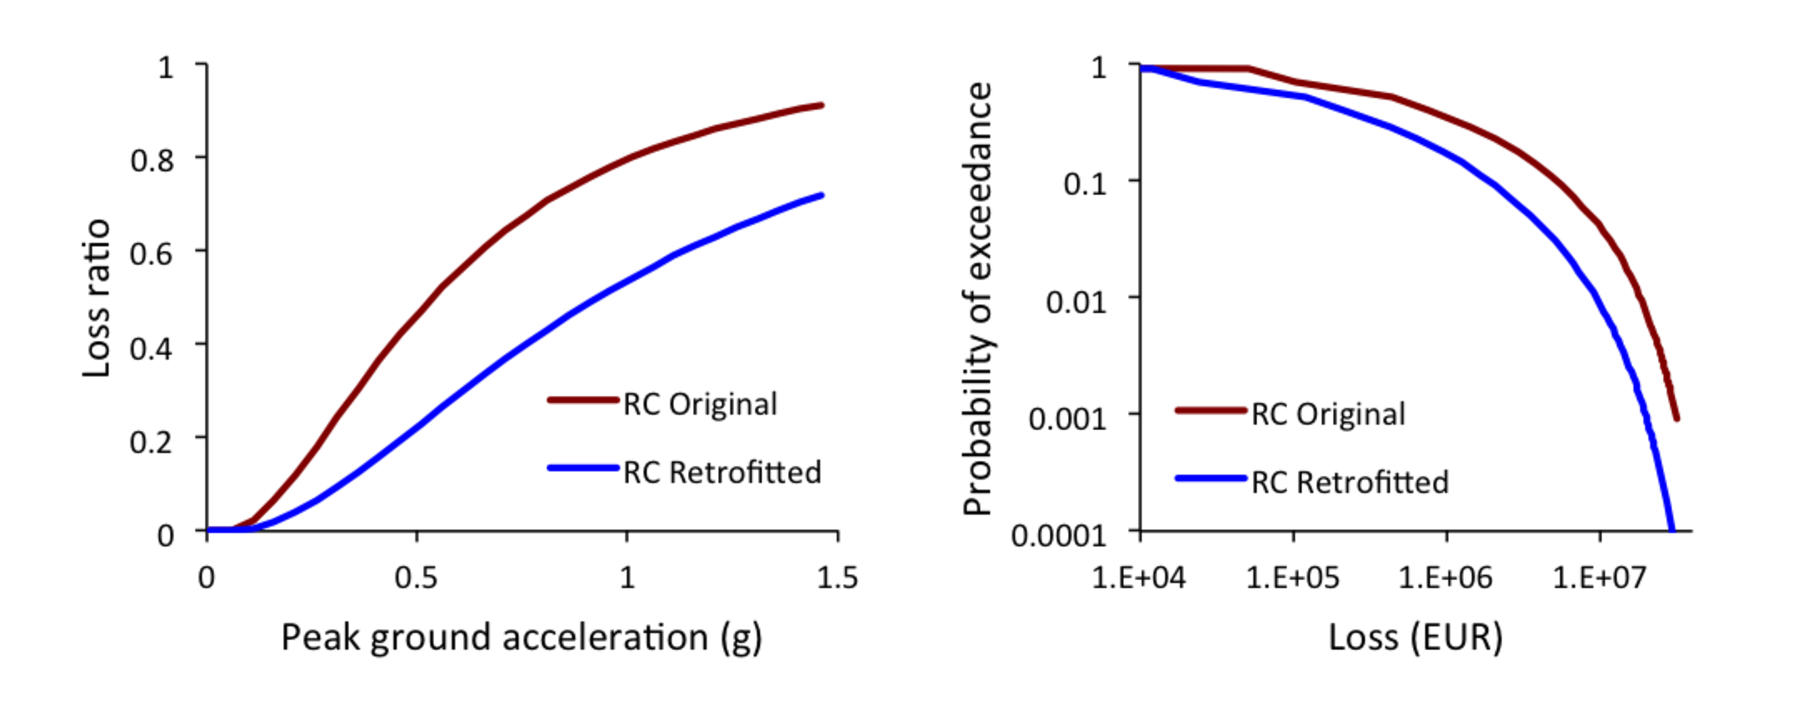
\includegraphics[width=12cm,height=5cm]{./figures/risk/VulnerabilityLosscurve.eps}
\caption{Vulnerability functions for the original and retrofitted configuration of a class of RC buildings (left) and respective loss exceedance curves (right).}
\label{fig:VulLosscurve}
\end{figure}

\item Then, an average annual loss ($AAL$) for each vulnerability configuration is calculated by numerically integrating the respective loss exceedance curve.  

\item For the calculation of the economic benefit $B$, the following formula can be employed:

\begin{equation}
B=(AAL_{retrofitted}-AAL_{original})\times\frac{1-e^{rt}}{r}
\end{equation}

where $r$ represents the discount rate, which serves the purposes of considering the variation of the economic value of the \glspl{asset} during their life expectancy, or design life ($t$).

\item Finally, the previously defined benefit ($B$) is divided by the retrofitting cost ($C$), leading to the benefit/cost ratio ($BCR$). This process is repeated for all the \glspl{asset} comprised in the \gls{exposure model}.

\end{enumerate}

\section{Calculator Output}
The results of this calculator are stored in a benefit/cost ratio map, which includes the $AAL_{retrofitted}$, $AAL_{original}$ and the resulting $BCR$ at each location. In Figure \ref{fig:BCRMap}, a map of benefit/cost ratios for RC residential buildings in Nepal is presented.

\begin{figure}[ht]
\centering
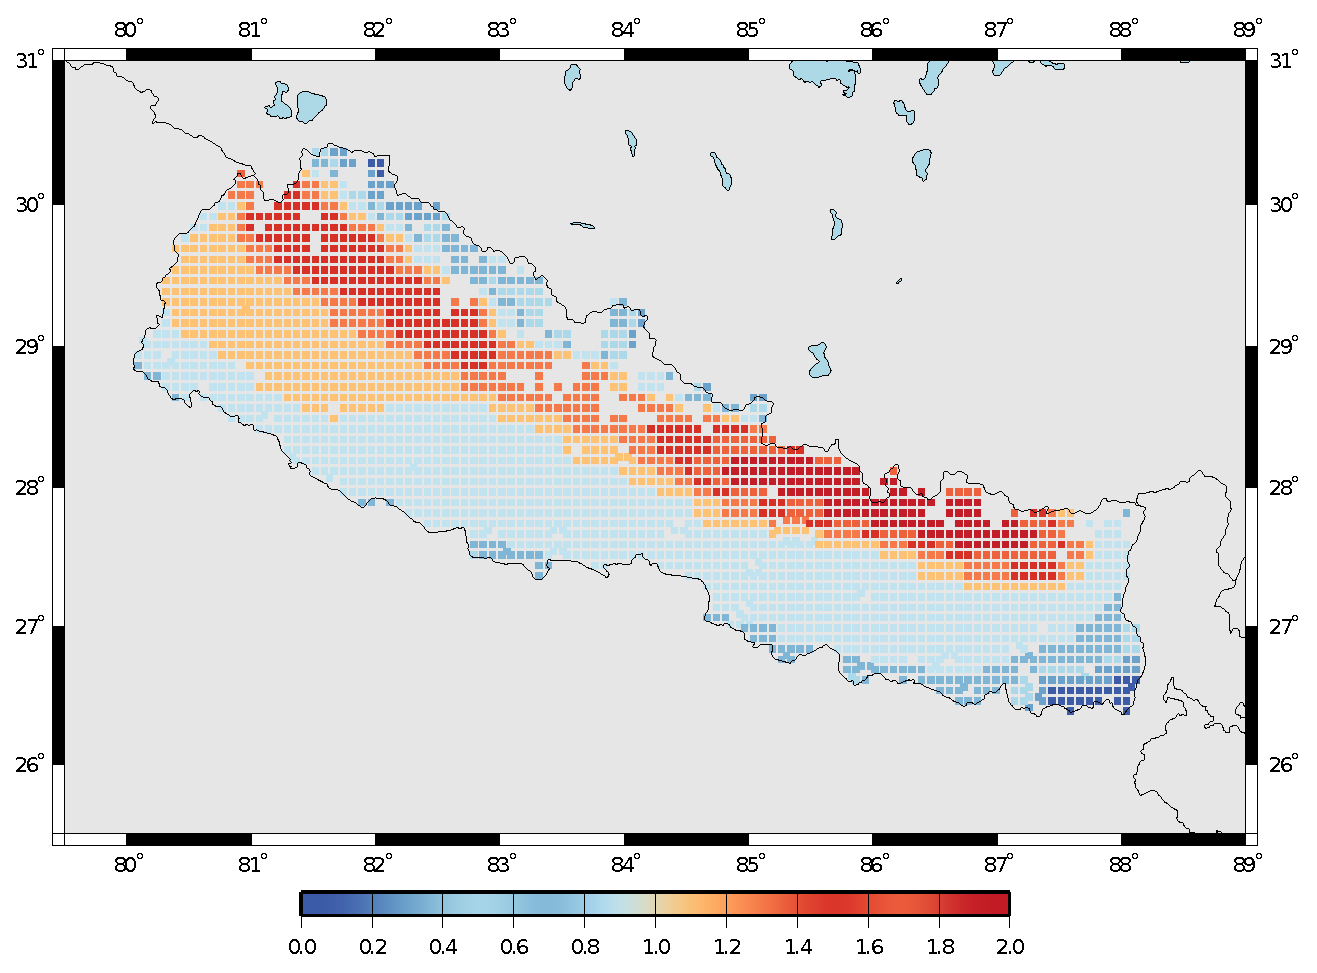
\includegraphics[width=12cm,height=8cm]{./figures/risk/BenefitCostRatioMap.eps}
\caption{Retrofitting benefit/cost ratio map for residential buildings in Nepal.}
\label{fig:BCRMap}
\end{figure}
% ==============================================================================
% ------------------------------------------------------------------------- Part
%\part{Socio-Economic Impact Assessment}
%	This book aims to provide an explanation of the scientific basis 
and the methodologies adopted in the implementation of the OpenQuake engine, an open source code for seismic hazard and physical risk calculation. 
%
The book follows the traditional openness and transparency features of the 
\gls{acr:gem} as clearly indicated in the development principles of 
the OpenQuake engine. 

%
The \gls{acr:gem} initiative is a global collaborative effort with the aim to provide organisations and people with tools and resources for transparent assessment of earthquake risk anywhere in the world.
%
The OpenQuake engine is a fully integrated, flexible and scalable hazard and physical risk 
calculation engine whose development is at the core of \gls{acr:gem}'s
overall objectives.
% ------------------------------------------------------------------------------
\section{Basics of the Engine}
The implementation of the OpenQuake software officially started in Summer 2010 
following the experience gained in \gls{acr:gem}'s kick-off project GEM1 
\citep{gemfoundation2010}, during which an extensive appraisal of existing hazard 
and physical risk codes was performed \citep{danciu2010,crowley2010}
and prototype hazard and risk software were selected, designed and
implemented \citep{pagani2010,crowley2010a}.

The current version of the OpenQuake engine is Python code developed 
following the most common requirements of Open Source 
software development, such as a public repository, IRC channel and open mailing lists. 
The source code, released under an open source software license,
is freely and openly accessible on a web based repository 
(see \href{http://github.com/gem}{github.com/gem}) while the 
development process is managed so that the community can participate 
to the day by day development as well as in the mid- and long-term 
design process. 
%
The software development also leverages on a number of open source projects 
such as \href {http://celeryproject.org}{Celeryd} and \href{http://www.rabbitmq.com}{RabbitMQ}, just to mention a few.

The hazard component of the engine largely relies on classes belonging to the OpenQuake Hazard library (see \href{https://github.com/gem/oq-hazardlib}{oq-hazardlib}) a comprehensive library for performing state-or-the-art PSHA. This library has been designed and implemented following the successful collaboration and important lessons learnt working with the \href{http://www.opensha.org}{OpenSHA} software and the developing teams at \gls{acr:usgs} and 
\gls{acr:scec} in GEM1. 
%
The risk component of the engine was designed in GEM1, prototyped in Java and eventually
coded in Python by the team operating at the \gls{acr:gem} 
Model Facility. This scientific code was originally integrated with the engine, but in late 2012 it was extracted to form the OpenQuake Risk Library (see \href{https://github.com/gem/oq-risklib}{oq-risklib}).

%A schema that illustrates the structure of the engine is 
%represented in Figure \ref{fig:openquake_schema}; the schema contains:
%purple boxes representing the main modules of the hazard component, 
%green boxes showing the modules of the risk component, white boxes
%with main outputs computed by the distinct modules and orange rectangles
%displaying the main input information that should be entered into the calculation engine. 
%
% ------------------------------------------------------------------------------
%\subsection{Brief description of the OpenQuake IT architecture}
%% ------------------------------------------------------------------------------
Openquake is the core of the OpenGEM system. 
%
As it appears in Figure \ref{fig:oq_it}, OpenQuake is powered by a 
number of open source software projects, of which OpenSHA-lite and 
RiskLib are currently the most essential ones. 
OpenSHA-lite is a ‘light’ version of the comprehensive software for 
probabilistic seismic hazard assessment OpenSHA and whose code serves
as a basis for the hazard component of the OpenQuake engine. RiskLib 
is a global collaboration project that is aimed at common development 
of a code ‘library’ for the risk all types of natural hazards, including
an API, on wh ich ‘apps’ can be built, such as tools that support risk
mitigation/reduction. The World Bank’s GFDRR, OpenGeo, AIFDR and GEM 
jointly work on RiskLib and its code repository, currently part of 
the OpenQuake project, will be broken out soon.
%
% . . . . . . . . . . . . . . . . . . . . . . . . . . . . . . . . . . . > Figure
\begin{figure}
\includegraphics[width=\textwidth,angle=0]{./Figures/Part_Introduction/oq_system_architecture.eps}
\caption{Openquake system architecture.}
\label{fig:oq_it}
\end{figure}
% . . . . . . . . . . . . . . . . . . . . . . . . . . . . . . . . . . . < Figure
%
Implementation of a standard format for data exchange for natural hazard
and risk,  is closely related to what is described above. The NRML 
(Natural hazards’ Risk Markup Language) format has been developed, which
is capable of encompassing a wide variety of risk and hazard data formats.
More information can be found in the detailed background documentation 
for OpenQuake.

The data services that are mentioned above are globally accessible 
read/write collaborations of core data sets that are exposed with a 
REST API. Some of the core modules of GEM will be available through 
the services and are currently being developed by GEM’s Model Facility 
development team, in collaboration with a number of IT partners and the 
scientists coordinating the modules. Examples are the development of a 
global exposure database, development of a global portal for active 
faults, global vulnerability functions and an earthquake consequences
database.






%
% ------------------------------------------------------------------------------
\section{Structure of the Book}
The OpenQuake Engine Book is organized into two volumes, one which describes the science behind the hazard component of the engine
and another which illustrates the theory of the physical risk calculators incorporated into the software. Readers that are interested in learning how to run calculations using the OpenQuake engine are referred to the OpenQuake Engine User Manual.

\hfill \\
%\emph{Part II: Hazard}
The GEM Hazard Team is currently updating the volume on hazard. In the meantime, interested readers are referred to the OpenQuake Engine User Manual, or they can contact the coordinator, Dr Marco Pagani, for further information. 
%\begin{itemize}
%\item Chapter \ref{chap:inthaz} offers an introduction to the hazard 
%topics discussed in the following chapters. In particular, in this 
%Chapter we discuss the main OpenQuake concepts and we illustrate the 
%calculation workflows currently available in the hazard component of 
%OpenQuake.
%\item Chapter \ref{chap:hazinp} focuses on the structure and the 
%characteristics of the information necessary to define a 
%comprehensive PSHA input model. This Chapter also includes
%descriptions of the main seismic source typologies and of the logic 
%tree structure.
%\item We dedicate Chapter \ref{chap:erf} to the explanation of the
%methodology adopted for the processing of the logic tree structures
%supported by OpenQuake and for the creation of the 
%\gls{earthquakeruptureforecast}
%\item The last Chapter of the hazard part (chapter \ref{chap:hazcalc}) 
%illustrates the main calculators available: the classical-PSHA calculator,
%the event-based calculator and the disaggregation calculator. 
%\end{itemize}
\hfill \\
\hfill \\
%\emph{Part III: Risk}
This volume on risk is organised as follows:
\begin{itemize}
\item Chapter \ref{chap:intrisk} introduces the main physical risk concepts and workflows. 
\item Chapter \ref{chap:riskinput} contains an explanation of the exposure, physical vulnerability and fragility concepts, which are input to the calculations.
\item Chapter \ref{chap:scenario_risk} describes the scenario risk 
methodology, for estimating loss distributions for single events.
\item Chapter \ref{chap:scenario_damage} describes the scenario damage 
methodology, for estimating damage ditributions for single events.
\item Chapter \ref{chap:risk_prob_event_based} provides an overview of the probabilistic event-based risk calculation methodology, which produces loss exceedance curves for portfolios of buildings.
\item Chapter \ref{chap:risk_psha_based} illustrates single-site risk calculations based on the hazard curves from classical PSHA.
\item Chapter \ref{chap:bcr} outlines the benefit/cost ratio calculations based on loss curves for structures with and without retrofitting.
\end{itemize}
%
%In the closing part, the Book contains a glossary that aims to define a 
%clear and unique terminology.
%
% . . . . . . . . . . . . . . . . . . . . . . . . . . . . . . . . . . . > Figure
%\begin{landscape}
%\begin{figure}
%\includegraphics[width=20cm,angle=0]{./Figures/Part_Introduction/engine9_20110130.eps}
%\caption{OpenQuake Engine schema. Purple boxes are the calculators included in the  
%the hazard part of OQ; green boxes are the physical risk calculators.}
%\label{fig:openquake_schema}
%\end{figure}
%\end{landscape}
% . . . . . . . . . . . . . . . . . . . . . . . . . . . . . . . . . . . < Figure
% ==============================================================================
% ------------------------------------------------------------------------- Part
%\part{Modeller's Toolkit}
% ------------------------------------------------------------------------------
%\chapter{Introduction}
%	This book aims to provide an explanation of the scientific basis 
and the methodologies adopted in the implementation of the OpenQuake engine, an open source code for seismic hazard and physical risk calculation. 
%
The book follows the traditional openness and transparency features of the 
\gls{acr:gem} as clearly indicated in the development principles of 
the OpenQuake engine. 

%
The \gls{acr:gem} initiative is a global collaborative effort with the aim to provide organisations and people with tools and resources for transparent assessment of earthquake risk anywhere in the world.
%
The OpenQuake engine is a fully integrated, flexible and scalable hazard and physical risk 
calculation engine whose development is at the core of \gls{acr:gem}'s
overall objectives.
% ------------------------------------------------------------------------------
\section{Basics of the Engine}
The implementation of the OpenQuake software officially started in Summer 2010 
following the experience gained in \gls{acr:gem}'s kick-off project GEM1 
\citep{gemfoundation2010}, during which an extensive appraisal of existing hazard 
and physical risk codes was performed \citep{danciu2010,crowley2010}
and prototype hazard and risk software were selected, designed and
implemented \citep{pagani2010,crowley2010a}.

The current version of the OpenQuake engine is Python code developed 
following the most common requirements of Open Source 
software development, such as a public repository, IRC channel and open mailing lists. 
The source code, released under an open source software license,
is freely and openly accessible on a web based repository 
(see \href{http://github.com/gem}{github.com/gem}) while the 
development process is managed so that the community can participate 
to the day by day development as well as in the mid- and long-term 
design process. 
%
The software development also leverages on a number of open source projects 
such as \href {http://celeryproject.org}{Celeryd} and \href{http://www.rabbitmq.com}{RabbitMQ}, just to mention a few.

The hazard component of the engine largely relies on classes belonging to the OpenQuake Hazard library (see \href{https://github.com/gem/oq-hazardlib}{oq-hazardlib}) a comprehensive library for performing state-or-the-art PSHA. This library has been designed and implemented following the successful collaboration and important lessons learnt working with the \href{http://www.opensha.org}{OpenSHA} software and the developing teams at \gls{acr:usgs} and 
\gls{acr:scec} in GEM1. 
%
The risk component of the engine was designed in GEM1, prototyped in Java and eventually
coded in Python by the team operating at the \gls{acr:gem} 
Model Facility. This scientific code was originally integrated with the engine, but in late 2012 it was extracted to form the OpenQuake Risk Library (see \href{https://github.com/gem/oq-risklib}{oq-risklib}).

%A schema that illustrates the structure of the engine is 
%represented in Figure \ref{fig:openquake_schema}; the schema contains:
%purple boxes representing the main modules of the hazard component, 
%green boxes showing the modules of the risk component, white boxes
%with main outputs computed by the distinct modules and orange rectangles
%displaying the main input information that should be entered into the calculation engine. 
%
% ------------------------------------------------------------------------------
%\subsection{Brief description of the OpenQuake IT architecture}
%% ------------------------------------------------------------------------------
Openquake is the core of the OpenGEM system. 
%
As it appears in Figure \ref{fig:oq_it}, OpenQuake is powered by a 
number of open source software projects, of which OpenSHA-lite and 
RiskLib are currently the most essential ones. 
OpenSHA-lite is a ‘light’ version of the comprehensive software for 
probabilistic seismic hazard assessment OpenSHA and whose code serves
as a basis for the hazard component of the OpenQuake engine. RiskLib 
is a global collaboration project that is aimed at common development 
of a code ‘library’ for the risk all types of natural hazards, including
an API, on wh ich ‘apps’ can be built, such as tools that support risk
mitigation/reduction. The World Bank’s GFDRR, OpenGeo, AIFDR and GEM 
jointly work on RiskLib and its code repository, currently part of 
the OpenQuake project, will be broken out soon.
%
% . . . . . . . . . . . . . . . . . . . . . . . . . . . . . . . . . . . > Figure
\begin{figure}
\includegraphics[width=\textwidth,angle=0]{./Figures/Part_Introduction/oq_system_architecture.eps}
\caption{Openquake system architecture.}
\label{fig:oq_it}
\end{figure}
% . . . . . . . . . . . . . . . . . . . . . . . . . . . . . . . . . . . < Figure
%
Implementation of a standard format for data exchange for natural hazard
and risk,  is closely related to what is described above. The NRML 
(Natural hazards’ Risk Markup Language) format has been developed, which
is capable of encompassing a wide variety of risk and hazard data formats.
More information can be found in the detailed background documentation 
for OpenQuake.

The data services that are mentioned above are globally accessible 
read/write collaborations of core data sets that are exposed with a 
REST API. Some of the core modules of GEM will be available through 
the services and are currently being developed by GEM’s Model Facility 
development team, in collaboration with a number of IT partners and the 
scientists coordinating the modules. Examples are the development of a 
global exposure database, development of a global portal for active 
faults, global vulnerability functions and an earthquake consequences
database.






%
% ------------------------------------------------------------------------------
\section{Structure of the Book}
The OpenQuake Engine Book is organized into two volumes, one which describes the science behind the hazard component of the engine
and another which illustrates the theory of the physical risk calculators incorporated into the software. Readers that are interested in learning how to run calculations using the OpenQuake engine are referred to the OpenQuake Engine User Manual.

\hfill \\
%\emph{Part II: Hazard}
The GEM Hazard Team is currently updating the volume on hazard. In the meantime, interested readers are referred to the OpenQuake Engine User Manual, or they can contact the coordinator, Dr Marco Pagani, for further information. 
%\begin{itemize}
%\item Chapter \ref{chap:inthaz} offers an introduction to the hazard 
%topics discussed in the following chapters. In particular, in this 
%Chapter we discuss the main OpenQuake concepts and we illustrate the 
%calculation workflows currently available in the hazard component of 
%OpenQuake.
%\item Chapter \ref{chap:hazinp} focuses on the structure and the 
%characteristics of the information necessary to define a 
%comprehensive PSHA input model. This Chapter also includes
%descriptions of the main seismic source typologies and of the logic 
%tree structure.
%\item We dedicate Chapter \ref{chap:erf} to the explanation of the
%methodology adopted for the processing of the logic tree structures
%supported by OpenQuake and for the creation of the 
%\gls{earthquakeruptureforecast}
%\item The last Chapter of the hazard part (chapter \ref{chap:hazcalc}) 
%illustrates the main calculators available: the classical-PSHA calculator,
%the event-based calculator and the disaggregation calculator. 
%\end{itemize}
\hfill \\
\hfill \\
%\emph{Part III: Risk}
This volume on risk is organised as follows:
\begin{itemize}
\item Chapter \ref{chap:intrisk} introduces the main physical risk concepts and workflows. 
\item Chapter \ref{chap:riskinput} contains an explanation of the exposure, physical vulnerability and fragility concepts, which are input to the calculations.
\item Chapter \ref{chap:scenario_risk} describes the scenario risk 
methodology, for estimating loss distributions for single events.
\item Chapter \ref{chap:scenario_damage} describes the scenario damage 
methodology, for estimating damage ditributions for single events.
\item Chapter \ref{chap:risk_prob_event_based} provides an overview of the probabilistic event-based risk calculation methodology, which produces loss exceedance curves for portfolios of buildings.
\item Chapter \ref{chap:risk_psha_based} illustrates single-site risk calculations based on the hazard curves from classical PSHA.
\item Chapter \ref{chap:bcr} outlines the benefit/cost ratio calculations based on loss curves for structures with and without retrofitting.
\end{itemize}
%
%In the closing part, the Book contains a glossary that aims to define a 
%clear and unique terminology.
%
% . . . . . . . . . . . . . . . . . . . . . . . . . . . . . . . . . . . > Figure
%\begin{landscape}
%\begin{figure}
%\includegraphics[width=20cm,angle=0]{./Figures/Part_Introduction/engine9_20110130.eps}
%\caption{OpenQuake Engine schema. Purple boxes are the calculators included in the  
%the hazard part of OQ; green boxes are the physical risk calculators.}
%\label{fig:openquake_schema}
%\end{figure}
%\end{landscape}
% . . . . . . . . . . . . . . . . . . . . . . . . . . . . . . . . . . . < Figure
% ------------------------------------------------------------------------------
%\chapter{Input visualization and preparation}
%	\input{./oqb/part_Modellers_Toolkit/input.tex}
% ==============================================================================
% ------------------------------------------------------------------------------
% ------------------------------------------------------------------------- Part
%\part{Appendixes}
%\appendix
% ------------------------------------------------------------------------------
%\chapter{nrML}
%	\input{./oqb/part_Appendix/nrML.tex}
% ------------------------------------------------------------------------------
%\chapter{Example of OpenQuake risk calculation configuration file}
%	\input{./oqb/part_Appendix/appendixHazardInputExample.tex}
% ==============================================================================
% ----------------------------------------------------------------- Bibliography
\small
\bibliographystyle{apalike}
\bibliography{./Bibliography/hazard,./Bibliography/risk,./Bibliography/sei.bib}
\normalsize
% ==============================================================================
% ------------------------------------------------------------------------ Index
\printglossaries
\printindex
\cleardoublepage
% Final empty page
\hfill \\ \thispagestyle{empty} \clearpage 
% ==============================================================================
% ------------------------------------------------------------------- Back Cover
\newgeometry{hmargin={0cm,-0.4cm},height=29.7cm}
\thispagestyle{empty}
\psset{unit=1cm}
\begin{pspicture}(0,0)(21cm,29.7cm)
	\psframe[fillstyle=solid,linecolor=cyan,fillcolor=white]
		(0.0cm,0.0cm)(21cm,15.0cm)
	\psframe[fillstyle=solid,linecolor=white,fillcolor=white]
		(0.0cm,15.0cm)(21cm,29.7cm)
	\psframe[fillstyle=solid,linecolor=blue01,fillcolor= blue01]
		(0.0cm,15.0cm)(21cm,15.5cm)
	\psframe[fillstyle=solid,linecolor=blue01,fillcolor= blue01]
		(0.0cm,25.0cm)(21cm,25.1cm)
\end{pspicture}
%
\end{document}
